\clearpage

\appendix

\section*{Appendix}

\addcontentsline{toc}{section}{Appendix}

\startcontents[appendix]

\printcontents[appendix]{}{1}{\section*{Contents}}

\clearpage

\counterwithin{figure}{section} % Binds figure numbering to the section (e.g., A.1)
\setcounter{figure}{0}          % Resets the figure counter to 0


\section{More Related Work}

\textbf{Definition for Generalist Robotics (GR)}
In FA, variations in the environment and object shape and pose are minimal. For GR, on the other hand, a robot performs a variety of different tasks (e.g., placing groceries into a refrigerator, or 
domestic cleaning, folding, kitchen pick-and-place) in different homes, where environments vary considerably and objects have variable geometry and highly variable initial poses. Recent robot learning research predominantly targets highly unstructured Generalist Robotics (GR), such as household robots executing diverse chores across novel environments using a single generalist model-free VLA policies~\cite{levine2016end, chi2025diffusion, kim24openvla, pi0_2024, black2025pi_}.


\textbf{Self-Improving Agentic Workflows}.
Outside of robotics, Large Language Models (LLMs) have demonstrated exceptional capabilities in dynamic coding, complex software integration, and API orchestration \cite{wu2024introducing, team2026qwen3, hou2025model, openai2024gpt4o, anthropic2024claude35, google2025gemini25}. By embedding these capabilities into structured agentic workflows, LLMs can autonomously synthesize solutions for open-ended tasks~\cite{zhang2025aflow}. A foundational example is Voyager \cite{wang2023voyager}, which uses LLMs to iteratively write, refine, and execute Minecraft game playing skills to continually expand a curated library of reusable skills. In these frameworks, a ``skill'' is typically defined as a discrete function with strict semantic contracts. Recent literature has begun to explore the iterative optimization of agentic systems through language-based failure reasoning \cite{zehle2026promptolution} and multi-agent prompt optimization frameworks \cite{agrawal2025gepa, lee2025feedback}.
% In the domain of robotics, an agentic tool-use paradigm translates into a dynamic sequencing and parameterization of model-based or model-free sensorimotor primitives. Early works successfully grounded LLM reasoning in robotic affordances \cite{ahn2022can, huang2022inner}, while frameworks such as 
To improve code generation quality and performance, CaP-X~\cite{fu2026cap} used a VLM to provide feedback before and after execution (i.e. Visual Differencing), but the VLM can suffer from hallucinations and cannot handle geometric and numerical information such as motion feasibility. 
Building on the structure of Blox-Net~\cite{goldberg2025bloxnet} and BrickGPT~\cite{pun2025brickgpt}, which uses physical experiments to improve LLM-generated task plans, GaP uses multiple LLM agents to generate a robot computation graph and iteratively improve it using simulation experiments.
% However, while these frameworks generate plausible open-loop plans, they often lack the physical grounding necessary to verify geometric and kinematic feasibility before real-world deployment. To address this reality gap, 



% \input{tables/skills}




\section{Integrating ROS with GaP in Cable Insertion Benchmark}

We demonstrate how GaP can integrate the ROS through a cable insertion benchmark. Four nodes (\textit{align to port}, \textit{touch port}, \textit{insert}, \textit{extract}) are exposed to GaP through an intermediate skill interface that manages and triggers the ROS nodes sequentially. Upon receiving a call from the Behavior Graph, the skill interface instantiates a temporary ``orchestrator'' node to handle communication with the target ROS node, waiting until it receives a success, failure, or data signal. This execution status is then returned to the Behavior Graph, which determines the next workflow step and triggers subsequent ROS nodes accordingly.

% how GaP performed when these skills were available

% Figure~\ref{fig:usb-insert-graph} left shows the human-engineered ROS computation graph. Figure~\ref{fig:usb-insert-graph} in the middle shows the GaP-generated graph using the ROS nodes that performs a similar workflow as a human-engineered one (i.e.,  Figure~\ref{fig:usb-insert-graph} left). The text prompt ``Insert USB-C cable into port 1 and then extract it. If insertion fails, try again from the beginning." was used for this. The same skill set can be used as a composite skill so that GaP creates the subgraph to complete a long-horizon task (e.g., ``Insert USB-C cable into ports in ascending order.").

% "Insert USB-C cable into port 1."
% "Insert USB-C cable into port 2."
% "Insert USB-C cable into port 4."
% "Insert USB-C cable into port 5."
% "Insert USB-C cable into port 7."
% "Insert USB-C cable in ascending order"
% "Insert USB-C cable in descending order"
% "Insert the USB-C cable into odd-numbered ports"
% "Insert the USB-C cable into even-numbered ports"


% "Insert USB-C cable into port 1 and then extract it. If insertion fails, try again. If it fails again, just exit."
% "Insert USB-C cable into port 1 and then extract it. If insertion fails, try again from the beginning. If it fails again, just exit."
% "Insert USB-C cable into port 1 and then extract it. If insertion fails, try again from the beginning."

\begin{figure}[b!]
    \centering
    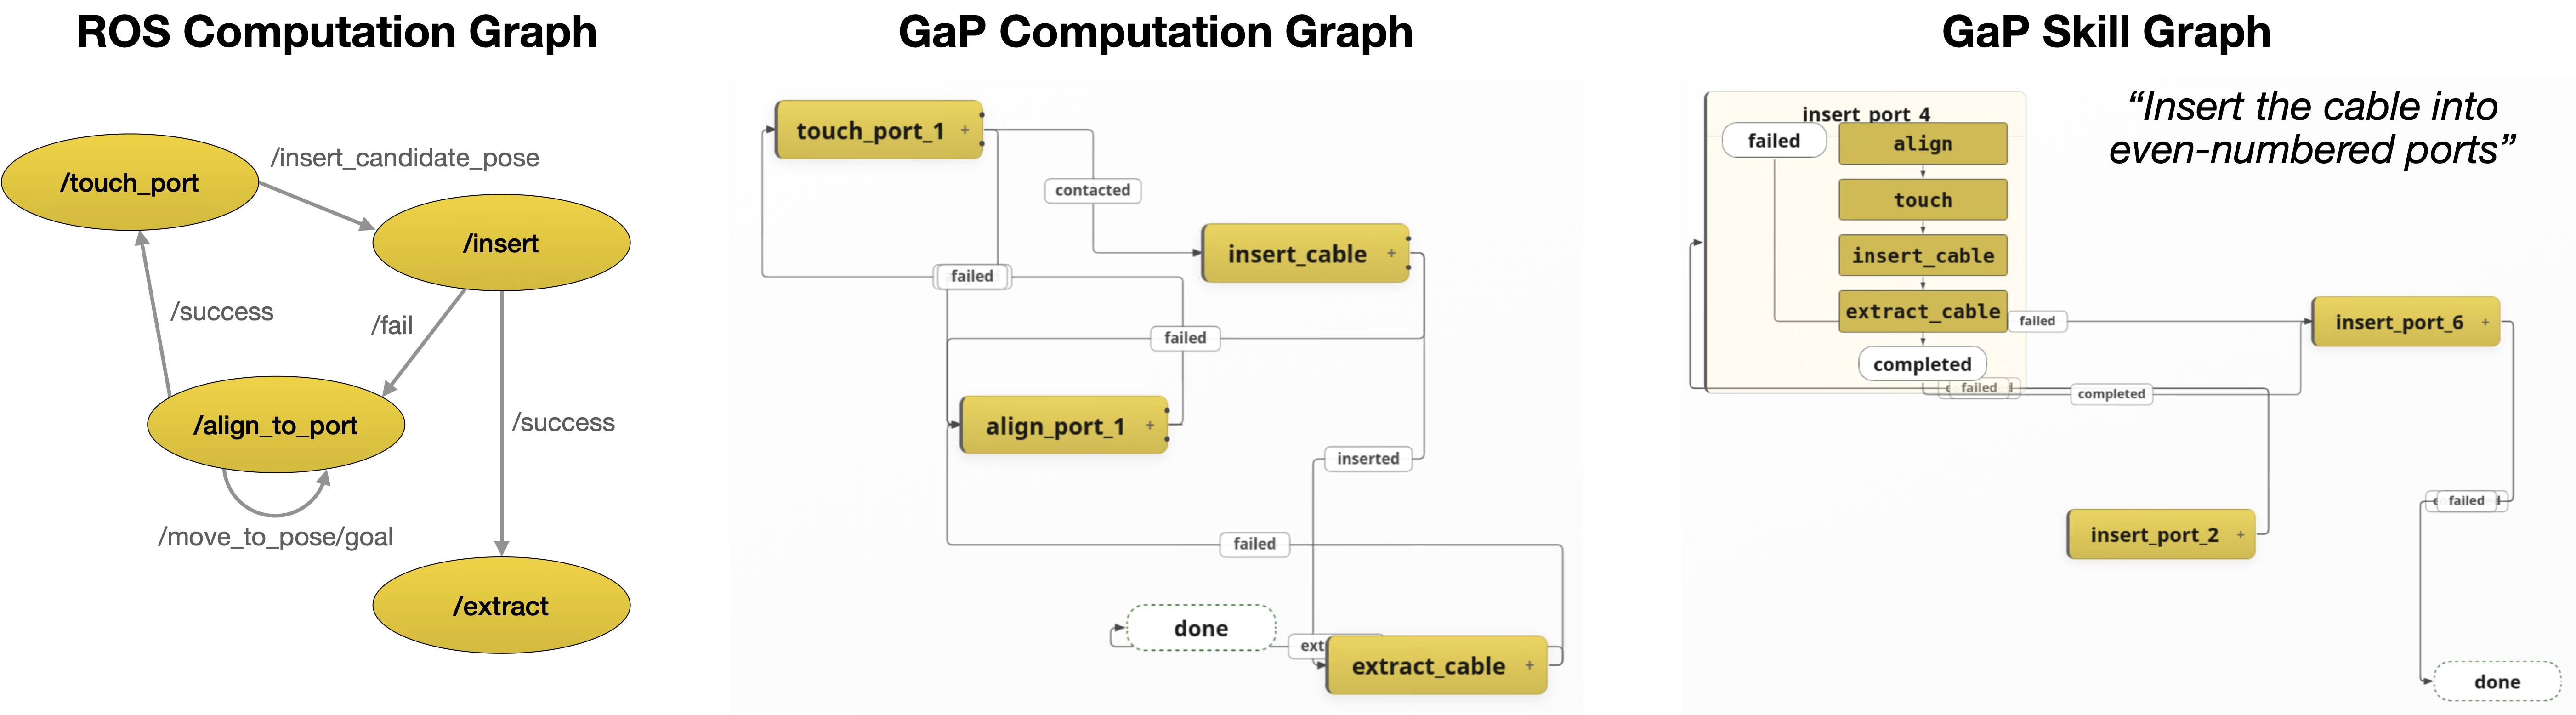
\includegraphics[width=1\linewidth]{figures/usb-insertion_graph.png}
    \caption{Left: ROS computation graph that is hand-engineered using traditional ROS nodes and topics. Middle: GaP can leverage nodes in ROS and generate a compatible graph using atomic skill sets, align to port, touch port, insert, and extract. Right: GaP can also use these nodes inside a subgraph for a long-horizon task, such as inserting the cable into even-numbered ports.}
    \label{fig:usb-insert-graph-app}
\end{figure}

\textbf{GaP provides flexibility to integrate with ROS nodes for robust, accurate task completion.} In our experiment, we create a computation graph using GaP with five different prompts: 1. individual port insertion ``Insert the cable into port X.'' (X: 1,2,4,5,7), 2. ``Insert the cable into ports in ascending order'', 3. ``Insert the cable into ports in descending order'', 4. ``Insert the cable into odd-indexed ports'', 5. ``Insert the cable into even-indexed ports''. Across 130 insertion trials, GaP achieved a 0.93 success rate (121/130). A detailed breakdown is provided in Table~\ref{tab:benchmark-insertion}. Some of the corresponding graphs generated by GaP are shown in Figure~\ref{fig:usb-insert-graph-app}. The framework successfully connected atomic skills to complete the core insertion task and demonstrated the capacity to generate subgraphs using these skills to handle extended long-horizon tasks. The GaP-created graph is comparable to an expert-engineered baseline graph built using traditional ROS nodes and topics (see the side-by-side comparison in Figure~\ref{fig:usb-insert-graph-app} left and middle). 

We identified three main failure modes in our insertion policy. First, when the initial vision-based insertion candidate fails, the system falls back to a contact-based search within a 1~$\times$~1~$cm^2$ area in 2~mm steps. If the initial vision estimate falls outside this search zone, the brute-force probing ultimately fails. Second, successful insertion requires precise alignment with the housing; inaccurate depth estimation occasionally results in only a partial insertion. Lastly, variable lighting conditions or shadows cast by the robot and housing can cause the initial port detection to fail.

% \section{Self Learning Pseudocode}
% \floatname{algorithm}{Self-Learning-Algorithm}
% % \subsection{Skill-aware graph update with Physical feedback}
% \begin{minipage}{\textwidth}
% \begin{algorithm}[H]
% \DontPrintSemicolon
% \caption{Rehearsal-based Graph Optimization}
% \label{alg:graph_opt}
% \SetKwInOut{KwInput}{In}
% \SetKwInOut{KwOutput}{Out}
% \noindent\textbf{Input:} $\mathcal{T} = \langle \mathcal{L}, \mathcal{E}, \mathcal{R}, \mathcal{O}, \mathcal{X}, \mathcal{B}, \mathcal{J} \rangle$,  Iterations $M$, Parallel Rollouts $N$ \\
% \noindent\textbf{Output:} Optimized Task Graph $\mathcal{G}^*$
% \BlankLine
% \textbf{Initialization:}\;
% $\mathcal{G}_0 \leftarrow \mathrm{Graph\_Init}(\mathcal{L})$\;
% \quad\tcp*[r]{ Initial graph from language}
% $\mathcal{S} \leftarrow \mathrm{Build\_Scene}(\mathcal{G}, \{\mathcal{G}_i\})$\;
% \quad\tcp*[r]{ Instantiate sim environment}
% \For{$j \leftarrow 1$ \KwTo $M$}{
%     \tcp{Step 1: Scene Variational Sampling}
%     $\{\hat{s}_i\}_{i=1}^N \sim \mathcal{B}$\;
%     \quad\tcp*[r]{ Sample $N$ instances}
%     \tcp{Step 2: Parallel Rehearsal}
%     \ParallelFor{$i \leftarrow 1$ \KwTo $N$}{
%         $\tau_i \leftarrow \mathrm{Rehearsal}(\hat{s}_i, \mathcal{G}_{j-1})$\;
%         \quad\tcp*[r]{ Rollout policy}
%         $F_i \leftarrow \mathrm{Analyze_\_Failure}(\tau_i, \mathcal{G}, \{\mathcal{G}_i\})$\;
    
%     }
%     \tcp{Step 3: Graph Refinement}
%     $\mathcal{G}_j \leftarrow \mathrm{Graph\_Update}(\{F_1, \dots, F_N\})$\;
%     \quad\tcp*[r]{ Optimize via LLM}
% }
% \Return $\mathcal{G}^* \leftarrow \mathcal{G}_M$\;
% \end{algorithm}
% \end{minipage}
% \vspace{-\baselineskip} 


% \newpage

\section{Sample Generated Graphs}

\subsection{Fulfill Grocery Orders}

\begin{figure}[H]
    \centering
    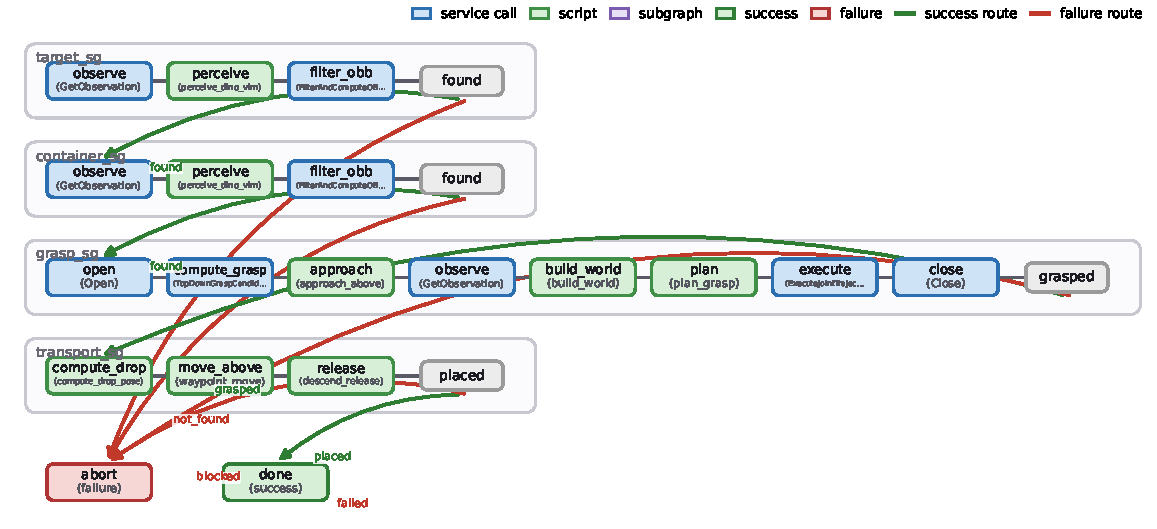
\includegraphics[width=0.98\linewidth]{graph_pdfs/posvar.pdf}
    % \caption{Caption}
    \label{fig:graph-posvar}
\end{figure}

\subsection{Pack Grocery Items}

\begin{figure}[H]
    \centering
    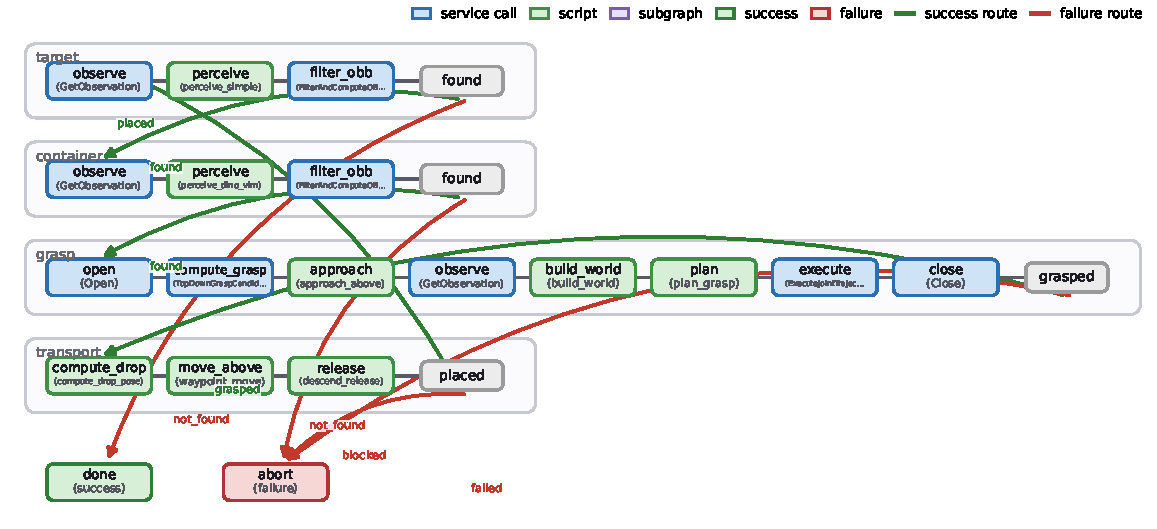
\includegraphics[width=0.98\linewidth]{graph_pdfs/packing.pdf}
    % \caption{Caption}
    \label{fig:graph-packing}
\end{figure}


\subsection{Fulfill Grocery Orders with VLA Policy}

\begin{figure}[H]
    \centering
    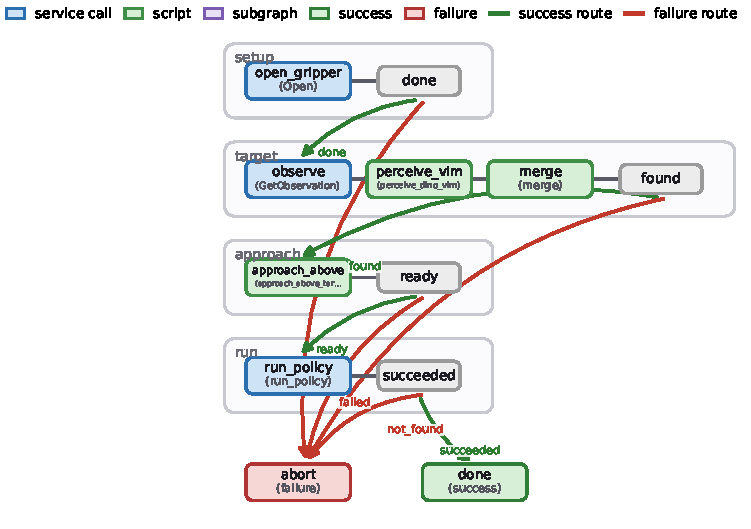
\includegraphics[width=0.9\linewidth]{graph_pdfs/popcorn.pdf}
    % \caption{Caption}
    \label{fig:graph-popcorn}
\end{figure}


\subsection{Wash Crates}

\begin{figure}[H]
    \centering
    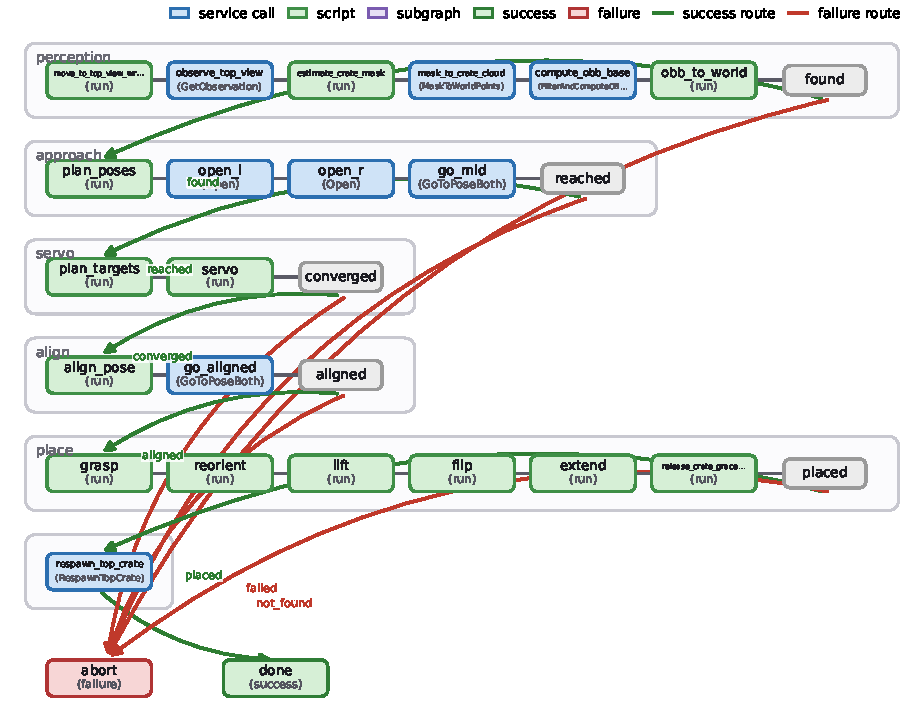
\includegraphics[width=\linewidth]{graph_pdfs/crate_washing_bosch.pdf}
    % \caption{Caption}
    \label{fig:graph-crate-washing}
\end{figure}

% \subsection{Fulfill Grocery Orders with VLA Policy}


\subsection{Make Popcorn}

\begin{figure}[H]
    \centering
    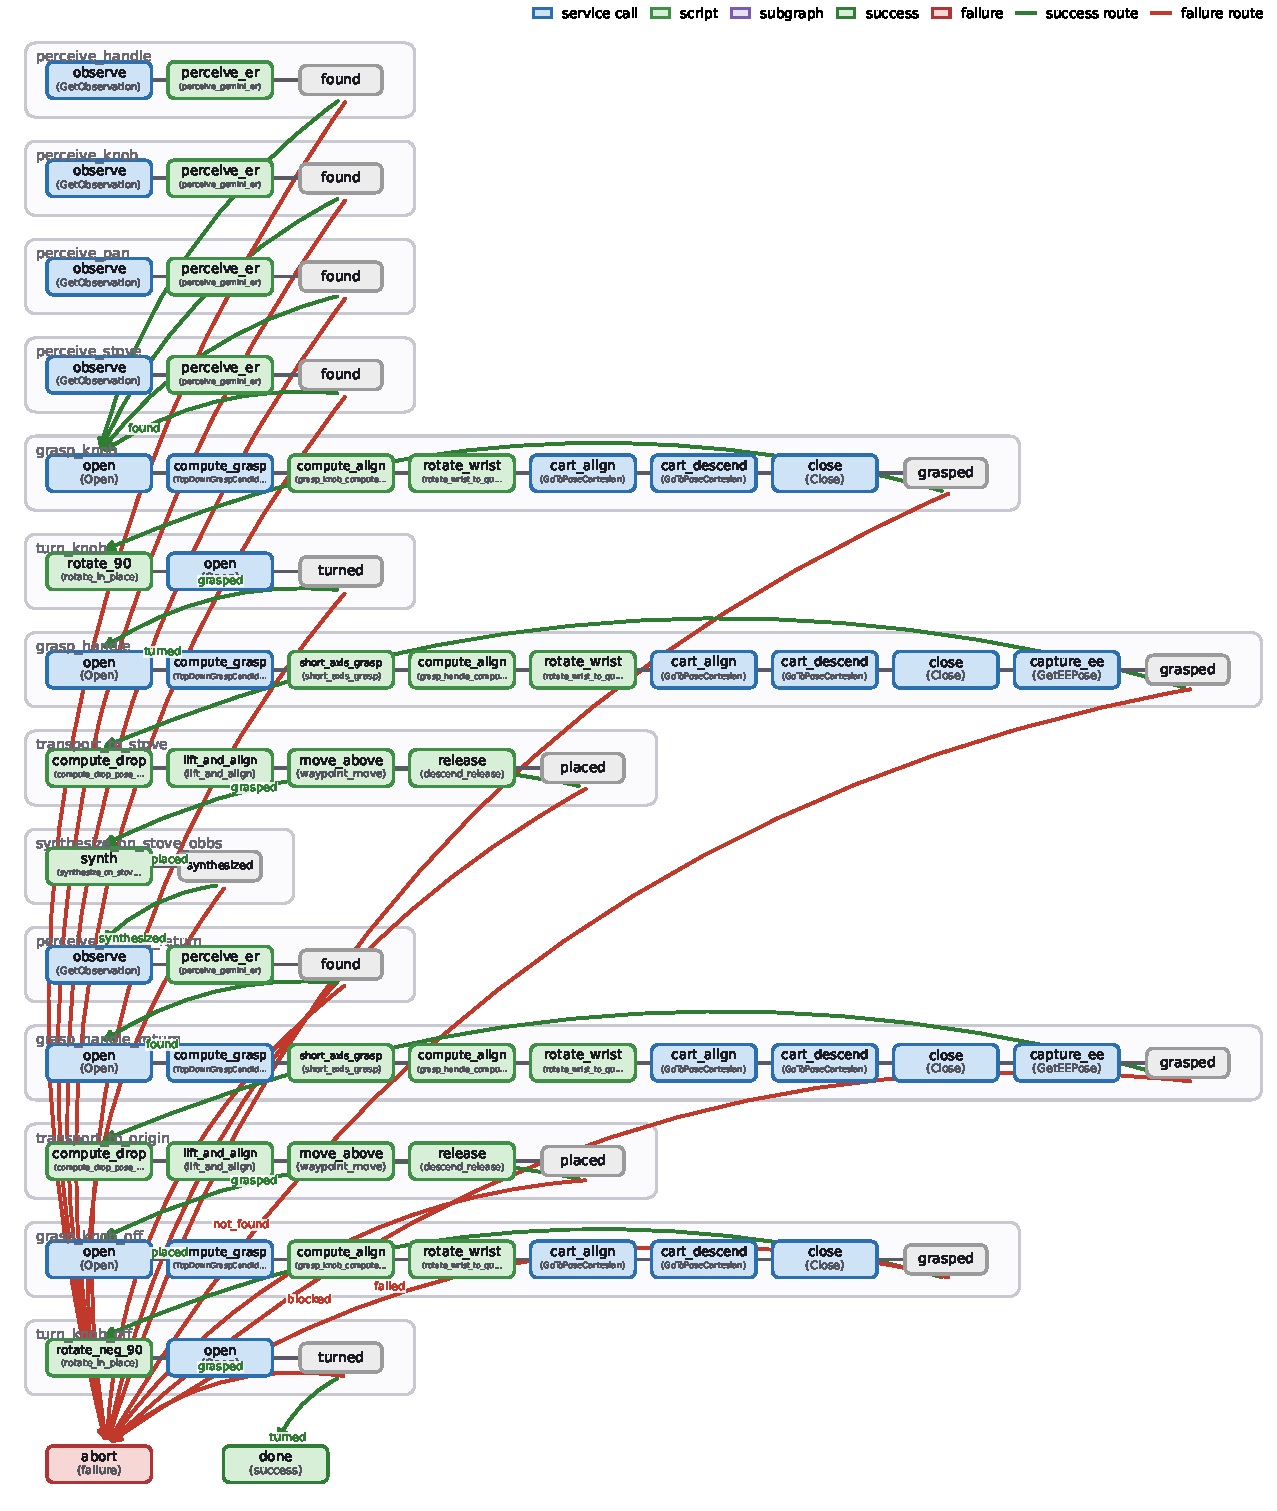
\includegraphics[width=\linewidth]{graph_pdfs/full_popcorn_cycle_cartesian.pdf}
    % \caption{Caption}
    \label{fig:graph-popcorn-full}
\end{figure}



\section{MORSL Library}
% =====================================================================
%  System Reference: Skills
%  Auto-generated from skills/*/SKILL.md and proto/*/v1/*.proto.
%  Regenerate when those change.
%
%  Composite/atomic skills are listed once. Every leaf gRPC method is
%  listed as its own skill (one RPC = one skill), with the request and
%  response fields drawn from its proto contract.
% =====================================================================
%
% Self-contained --- no extra packages required.
%
% \skillcard{name}{inputs}{outputs}{description}


The system is built from a single kind of component, the \emph{skill}.
Every skill is declared by the same metadata schema --- a name, a
description, and its typed inputs and outputs. Higher-level
\emph{composite} skills are materializable subgraphs authored by
composing other skills; \emph{atomic} skills are single classes; and
\emph{primitive} skills are individual gRPC methods, each wrapping one
model invocation or geometric routine. All skills share a common type
system (\texttt{Se3Pose}, \texttt{OrientedBoundingBox},
\texttt{PointCloud}, \texttt{Mask}, \texttt{Image}, \texttt{Trajectory},
\texttt{JointState}, $\dots$), which is what lets them compose freely. In
the input lists below, defaults are given in parentheses and the
universal caller-context field is omitted.

% =====================================================================
\subsection{Composite and atomic skills}




\paragraph{Perception.}

\skillcard{perception\_single}
{\texttt{object\_name} (literal)}
{\texttt{<name>\_obb}: OrientedBoundingBox, \texttt{<name>\_mask}: Mask, \texttt{<name>\_cloud}: PointCloud}
{Fast single-path detection: broad detect + a VLM crop tournament +
segmentation + depth-to-3D fusion, closed by an OBB fit. Best for
uncluttered scenes with visually distinct targets.}

\skillcard{perception\_multi}
{\texttt{object\_name} (literal)}
{\texttt{<name>\_obb}: OrientedBoundingBox, \texttt{<name>\_mask}: Mask}
{Three detectors run on the same observation and a VLM disambiguator picks
the best mask on disagreement. Most robust, but slower; single-shot only.}

\skillcard{perception\_any}
{\texttt{object\_name} (literal)}
{\texttt{<name>\_obb}: OrientedBoundingBox, \texttt{<name>\_mask}: Mask, \texttt{<name>\_cloud}: PointCloud}
{Lightweight one-shot set-of-marks pick. Returns ``not found'' cleanly
when the VLM replies ``none'', the right choice for clean-all-items loops.}

\skillcard{perception\_subpart}
{\texttt{parent\_prompt}, \texttt{subpart\_prompt} (literals)}
{\texttt{<name>\_obb}: OrientedBoundingBox, \texttt{<name>\_mask}: Mask, \texttt{<name>\_cloud}: PointCloud}
{Hierarchical perception: detect the parent, crop to its box, segment the
named subpart inside the crop, uncrop and fuse depth. For affordances that
occupy few full-image pixels (pan handle, drawer pull, mug rim).}

\skillcard{track\_object}
{text prompt; observation stream}
{a stream of tracked-mask snapshots}
{Long-running tracker: seeds on the first frame via text prompt, then polls
the observation stream and advances the tracker until the workflow signals
termination, freeing tracker state on exit.}

\paragraph{Grasping.}

\skillcard{grasp\_curobo\_obb}
{\texttt{target\_obb}: OrientedBoundingBox, \texttt{target\_mask}: Mask}
{\texttt{ee\_pose\_at\_grasp}: Se3Pose, \texttt{grasp\_pose}: Se3Pose}
{Collision-aware grasping: plans a collision-free trajectory to one of
several top-down OBB grasp candidates. The default when the OBB centroid
is graspable.}

\skillcard{grasp\_moe}
{\texttt{target\_obb}: OrientedBoundingBox, \texttt{target\_mask}: Mask, \texttt{target\_cloud}: PointCloud}
{\texttt{ee\_pose\_at\_grasp}: Se3Pose}
{Mixture-of-experts grasping: a diffusion sampler and a dense OBB sweep
feed one discriminator; the top-K union is planned. Use when the OBB
centroid is not the graspable point (bowl rim, handle, off-center).}

\skillcard{grasp\_short\_axis}
{\texttt{target\_obb}: OrientedBoundingBox, \texttt{target\_mask}: Mask, \texttt{base\_obb}: OrientedBoundingBox (optional)}
{\texttt{ee\_pose\_at\_grasp}: Se3Pose, \texttt{grasp\_pose}: Se3Pose}
{Deterministic geometry-locked grasp: the finger axis snaps to the OBB's
shorter horizontal axis so the jaws close across the narrow dimension of
an elongated target. An optional base OBB slides the grasp along a handle.}

\skillcard{grasp\_direct\_ik}
{\texttt{target\_obb}: OrientedBoundingBox}
{(grasp completion only)}
{Planner-free grasping: pre-rotate to the grasp orientation above the
target, descend straight down, close. For uncluttered scenes or platforms
without a motion planner.}

\paragraph{Transport, policy, and bimanual.}

\skillcard{transport\_to\_drop}
{\texttt{container\_obb}, \texttt{container\_mask}, \texttt{target\_obb}, \texttt{target\_mask}, \texttt{ee\_pose\_at\_grasp}}
{(placement completion only)}
{Moves a held object above a destination container and releases it. An
optional VLM-grounded step localizes a natural-language sub-region (``the
left compartment'') before the drop pose is computed.}

\skillcard{run\_policy}
{observation stream; \texttt{max\_windows}}
{(policy rollout completion)}
{Runs a learned VLA policy in closed loop, reading the observation stream
each window, until a VLM termination check fires or \texttt{max\_windows}
is reached.}

\skillcard{bimanual\_crate\_lift}
{(none --- waypoints are baked parameters)}
{\texttt{done}: bool, \texttt{final\_left\_world\_pos}, \texttt{final\_right\_world\_pos}}
{Two-arm crate lift: both arms side-grasp the crate's handle bars and raise
it in lock-step, in a fixed phase order
(open\,$\to$\,approach\,$\to$\,insert\,$\to$\,close\,$\to$\,lift\,$\to$\,settle).}

% =====================================================================
\subsection{Primitive skills (one per gRPC method)}

\paragraph{Detection and segmentation.}

\skillcard{grounding\_dino.Detect}
{\texttt{image}: Image; \texttt{text\_prompt} (period-separated phrases); \texttt{box\_threshold} (0.20); \texttt{text\_threshold} (0.20)}
{\texttt{detections}: [\,box: BoundingBox2D, label, score\,]}
{Zero-shot object detection from a text prompt; returns boxes, labels, and
confidence scores.}

\skillcard{owlvit.Detect}
{\texttt{image}: Image; \texttt{text\_queries}: string[]; \texttt{score\_threshold} (0.05)}
{\texttt{detections}: [\,box: BoundingBox2D, label, score\,]}
{Open-vocabulary object detection from a list of text queries; an
alternative to grounding\_dino.}

\skillcard{sam3.SegmentText}
{\texttt{image}: Image; \texttt{text\_prompt}}
{\texttt{masks}: Mask[], \texttt{scores}: float[], \texttt{boxes}: BoundingBox2D[]}
{Segment all instances matching a text description.}

\skillcard{sam3.SegmentPoint}
{\texttt{image}: Image; \texttt{pixel\_x}, \texttt{pixel\_y}}
{\texttt{masks}: Mask[], \texttt{scores}: float[]}
{Segment the object under a single pixel coordinate.}

\skillcard{sam3.SegmentBox}
{\texttt{image}: Image; \texttt{box}: BoundingBox2D; \texttt{pixel\_x}/\texttt{pixel\_y} + \texttt{use\_point} (false, optional foreground point)}
{\texttt{masks}: Mask[], \texttt{scores}: float[]}
{Segment within a bounding box, optionally refined by a foreground point.}

\skillcard{sam2.SegmentBox}
{\texttt{image}: Image; \texttt{box}: BoundingBox2D; \texttt{max\_masks} (0 = unlimited)}
{\texttt{masks}: Mask[], \texttt{scores}: float[]}
{Box-prompted segmentation (lighter SAM2 backend).}

\skillcard{sam2.SegmentPoint}
{\texttt{image}: Image; \texttt{pixel\_x}, \texttt{pixel\_y}}
{\texttt{masks}: Mask[], \texttt{scores}: float[]}
{Point-prompted segmentation (lighter SAM2 backend).}

\skillcard{sam3\_tracker.InitTracker}
{\texttt{image}: Image (first frame); one of \texttt{text} / \texttt{box} / point (\texttt{pixel\_x},\texttt{pixel\_y},\texttt{use\_point}); \texttt{object\_name}}
{\texttt{tracker\_id}, \texttt{initial\_mask}: Mask, \texttt{initial\_box}, \texttt{score}, \texttt{object\_present}}
{Initialize a stateful tracker session seeded with one frame and a prompt.}

\skillcard{sam3\_tracker.UpdateTracker}
{\texttt{tracker\_id}; \texttt{image}: Image (new frame)}
{\texttt{mask}: Mask, \texttt{box}, \texttt{confidence}, \texttt{object\_present}}
{Advance an existing tracker session by one frame.}

\skillcard{sam3\_tracker.CloseTracker}
{\texttt{tracker\_id}}
{(empty)}
{Free a tracker session; idempotent.}

\skillcard{sam3d.GenerateMesh}
{\texttt{object\_name}; \texttt{views}: [rgb, mask, intrinsics, camera\_pose]; \texttt{obb}: OrientedBoundingBox; \texttt{view\_selection}; \texttt{seed} (42); \texttt{output\_dir}}
{\texttt{mesh\_path}, \texttt{texture\_path}, \texttt{world\_pose}: Se3Pose, \texttt{scale}: Vec3, \texttt{chosen\_view\_index}, \texttt{num\_vertices}, \texttt{num\_faces}}
{Reconstruct a triangle mesh from an RGB image + mask, scaled and posed
into world frame via the OBB; writes an \texttt{.obj} for the rehearsal sandbox.}

\paragraph{Vision--language.}

\skillcard{molmo.PointPrompt}
{\texttt{image}: Image; \texttt{object\_name}}
{\texttt{pixel\_x}, \texttt{pixel\_y}, \texttt{found}}
{Point to a named object; returns pixel coordinates.}

\skillcard{molmo.Query}
{\texttt{prompt}; \texttt{image}: Image (optional); \texttt{use\_multiview}}
{\texttt{text}}
{Free-form visual question answering (Molmo backend).}

\skillcard{molmo.QueryYesNo}
{\texttt{prompt}; \texttt{image}: Image (optional); \texttt{use\_multiview}}
{\texttt{answer}: bool}
{Yes/no visual question answering (Molmo backend).}

\skillcard{vlm.Query}
{\texttt{prompt}; \texttt{image}: Image (optional)}
{\texttt{text}}
{Free-form visual question answering (configurable VLM backend).}

\skillcard{vlm.QueryYesNo}
{\texttt{prompt}; \texttt{image}: Image (optional)}
{\texttt{answer}: bool}
{Yes/no visual question answering (configurable VLM backend).}

\paragraph{Grasp generation.}

\skillcard{graspgen.PlanFromPointCloud}
{\texttt{target\_cloud}: PointCloud; \texttt{scene\_cloud} (optional); \texttt{num\_grasps} (200); \texttt{topk\_num\_grasps} (50); \texttt{grasp\_threshold} ($-1$); \texttt{remove\_outliers} (true)}
{\texttt{grasp\_poses}: Se3Pose[], \texttt{scores}: float[], \texttt{contact\_points}: Vec3[]}
{Diffusion-based 6-DoF grasp sampling from an object-segmented cloud;
ranked, world-frame, fingertip convention.}

\skillcard{graspgen.ScoreGrasps}
{\texttt{target\_cloud}: PointCloud; \texttt{candidate\_poses}: Se3Pose[]}
{\texttt{scores}: float[] (aligned to candidates)}
{Score caller-provided grasps with GraspGen's discriminator, so
OBB-sampled candidates are comparable with diffusion samples.}

\skillcard{graspnet.PlanFromDepth}
{\texttt{depth}: DepthImage; \texttt{intrinsics}: Matrix3x3; \texttt{segmentation}: Mask; \texttt{instance\_id}; knobs (\texttt{z\_min} 0.2, \texttt{z\_max} 2.0, \texttt{max\_retries} 7, $\dots$); optional wrist camera}
{\texttt{grasp\_poses}: Se3Pose[], \texttt{scores}: float[], \texttt{contact\_points}: Vec3[]}
{Contact-GraspNet 6-DoF grasp detection from a depth image + instance mask.}

\skillcard{graspnet.PlanFromPointCloud}
{\texttt{full\_cloud}: PointCloud; \texttt{segment\_cloud}: PointCloud; \texttt{instance\_id}; same knobs}
{\texttt{grasp\_poses}: Se3Pose[], \texttt{scores}: float[], \texttt{contact\_points}: Vec3[]}
{Contact-GraspNet grasp detection from precomputed clouds.}

\skillcard{m2t2.PlanFromPointCloud}
{\texttt{scene\_cloud}: PointCloud; \texttt{target\_cloud} (optional); \texttt{num\_points} (16384); \texttt{grasp\_threshold} (0.035); \texttt{max\_grasps} (200)}
{\texttt{grasp\_poses}: Se3Pose[], \texttt{scores}: float[], \texttt{contact\_points}: Vec3[]}
{M2T2 6-DoF grasp generation from a colored scene cloud; an alternative
candidate source.}

\paragraph{Motion planning and IK.}

\skillcard{curobo.PlanToGraspPoses}
{\texttt{world\_config}: WorldConfig; \texttt{start\_joint\_position}: JointState; \texttt{grasp\_poses}: Se3Pose[]; thresholds + collision knobs}
{\texttt{success}, \texttt{trajectory}: Trajectory, \texttt{goalset\_index}}
{Plan a collision-free trajectory to one of several grasp poses (goalset).}

\skillcard{curobo.PlanWithGraspedObject}
{\texttt{world\_config}; \texttt{start\_joint\_position}; \texttt{target\_pose}: Se3Pose; \texttt{object\_name}}
{\texttt{success}, \texttt{trajectory}: Trajectory}
{Plan a collision-free trajectory while holding a named grasped object.}

\skillcard{curobo.PlanLinear}
{\texttt{start\_pose}, \texttt{end\_pose}: Se3Pose; \texttt{start\_joint\_position}; \texttt{world\_config} (optional); \texttt{num\_waypoints} (20); \texttt{hold\_vec\_weight}}
{\texttt{success}, \texttt{trajectory}: Trajectory, \texttt{failure\_reason}}
{GPU-accelerated straight-line Cartesian motion via per-waypoint IK,
optionally constrained and collision-checked.}

\skillcard{curobo.PlanDirectedLinear}
{\texttt{start\_joint\_position}; \texttt{start\_pose}, \texttt{target\_pose}; \texttt{allowed\_axes}; \texttt{endpoint\_mode}; \texttt{orientation\_mode}}
{\texttt{success}, \texttt{trajectory}: Trajectory, \texttt{failure\_reason}}
{Constrained linear motion that holds selected Cartesian axes
(project-to-target / fixed-distance / orient-in-place).}

\skillcard{curobo.PlanGraspMotion}
{\texttt{start\_joint\_position}; \texttt{grasp\_pose}: Se3Pose; approach axis+distance (0.12); lift axis+distance (0.20)}
{\texttt{success}; \texttt{approach\_trajectory}, \texttt{grasp\_trajectory}, \texttt{lift\_trajectory}: Trajectory; \texttt{failure\_reason}}
{Three-phase grasp plan (free-space approach, constrained grasp,
constrained lift) so the caller can interleave gripper commands. (CuRobo v0.8.)}

\skillcard{curobo.SolveIK}
{\texttt{target\_pose}: Se3Pose; \texttt{seed\_config} (optional); \texttt{tcp\_offset}; \texttt{num\_seeds} (32)}
{\texttt{success}, \texttt{joint\_config}: JointState}
{Pure geometric IK for a single TCP pose (no world collision).}

\skillcard{curobo.PlanToPose}
{\texttt{target\_pose}: Se3Pose; \texttt{start\_joint\_position}; \texttt{world\_config} (optional); \texttt{tcp\_offset}}
{\texttt{success}, \texttt{trajectory}: Trajectory}
{Collision-aware trajectory to a single EE target pose.}

\skillcard{curobo.BatchGraspFeasibility}
{\texttt{world\_config}; \texttt{start\_state}: JointState; \texttt{grasp\_poses}: Se3Pose[]; \texttt{approach\_offset\_m} (0.10); \texttt{ignore\_obstacle\_names}}
{\texttt{feasible}: bool[], \texttt{grasp\_ik\_ok}: bool[], \texttt{approach\_ik\_ok}: bool[], \texttt{corridor\_collision\_fraction}: float[] (all aligned to input)}
{Per-pose scene-collision feasibility for a batch of grasp candidates;
filters blocked grasps before planning.}

\skillcard{curobo.ValidateJointTrajectoryRobot}
{\texttt{world\_config}; \texttt{trajectory}: Trajectory; collision knobs}
{\texttt{success}, \texttt{failure\_reason}, \texttt{first\_collision\_waypoint}, \texttt{collision\_status\_detail}}
{Validate joint waypoints against world + self-collision.}

\skillcard{curobo.ValidateJointTrajectoryGrasped}
{\texttt{world\_config}; \texttt{trajectory}; \texttt{object\_name}; collision knobs}
{\texttt{success}, \texttt{failure\_reason}, \texttt{first\_collision\_waypoint}, \texttt{collision\_status\_detail}}
{As above, with a grasped object attached at the first waypoint.}

\skillcard{pyroki.SolveIK}
{\texttt{target\_pose}: Se3Pose; \texttt{target\_link\_name} (panda\_hand); \texttt{prev\_config} (optional); \texttt{tcp\_offset} ($0,0,-0.1$)}
{\texttt{joint\_config}: JointState, \texttt{success}}
{CPU differentiable IK for a target EE pose; the planner-free IK fallback.}

\skillcard{pyroki.PlanLinear}
{\texttt{start\_pose}, \texttt{end\_pose}: Se3Pose; \texttt{num\_waypoints} (20); \texttt{dt} (0.02)}
{\texttt{trajectory}: Trajectory, \texttt{success}}
{CPU linear Cartesian trajectory between two poses.}

\paragraph{Geometry.}

\skillcard{geometry\_svc.FilterNoise}
{\texttt{point\_cloud}: PointCloud; \texttt{eps} (0.005); \texttt{min\_samples} (10)}
{PointCloud}
{DBSCAN noise filtering of a point cloud.}

\skillcard{geometry\_svc.ComputeOBB}
{\texttt{point\_cloud}: PointCloud}
{OrientedBoundingBox}
{Fit an oriented bounding box to 3D points.}

\skillcard{geometry\_svc.FilterAndComputeOBB}
{\texttt{point\_cloud}: PointCloud; \texttt{eps} (0.005); \texttt{min\_samples} (10)}
{OrientedBoundingBox}
{FilterNoise + ComputeOBB in one round trip.}

\skillcard{geometry\_svc.TopDownGraspFromOBB}
{\texttt{obb}: OrientedBoundingBox; \texttt{z\_offset}}
{Se3Pose}
{A single top-down grasp pose from an OBB.}

\skillcard{geometry\_svc.TopDownGraspCandidates}
{\texttt{obb}: OrientedBoundingBox; \texttt{z\_offset}}
{\texttt{poses}: Se3Pose[] (primary + 90$^\circ$-rotated)}
{Candidate top-down grasps so a planner can pick a reachable one.}

\skillcard{geometry\_svc.SelectTopDownGrasp}
{\texttt{grasp\_poses}: Se3Pose[]; \texttt{gripper\_position}: Vec3}
{Se3Pose}
{Pick the most top-down (and nearest) grasp from candidates.}

\skillcard{geometry\_svc.FrontGraspFromOBB}
{\texttt{obb}: OrientedBoundingBox; \texttt{approach\_offset} (0.08); \texttt{approach\_hint}; \texttt{z\_offset}}
{\texttt{grasp\_pose}, \texttt{pre\_grasp\_pose}: Se3Pose; \texttt{approach\_direction}, \texttt{slide\_axis}: Vec3}
{Front/horizontal grasp for a handle (drawers, doors), with a slide axis.}

\skillcard{geometry\_svc.DepthToPointCloud}
{\texttt{depth}: DepthImage; \texttt{intrinsics}: Matrix3x3}
{PointCloud (camera frame)}
{Back-project a depth image to a camera-frame point cloud.}

\skillcard{geometry\_svc.MaskToWorldPoints}
{\texttt{mask}: Mask; \texttt{depth}: DepthImage; \texttt{intrinsics}: Matrix3x3; \texttt{camera\_pose}: Se3Pose}
{PointCloud (world frame)}
{Back-project a 2D mask to world-frame 3D points.}

\skillcard{geometry\_svc.PixelToWorldPoint}
{\texttt{pixel\_x}, \texttt{pixel\_y}; \texttt{depth}; \texttt{intrinsics}; \texttt{camera\_pose}}
{Vec3 (world point)}
{Back-project a single pixel to a world point.}

\skillcard{geometry\_svc.TransformPoints}
{\texttt{point\_cloud}: PointCloud; \texttt{transform}: Se3Pose}
{PointCloud}
{Apply a rigid transform to a set of points.}

\skillcard{geometry\_svc.BuildWorldConfig}
{\texttt{cameras}: CameraObservation[]; \texttt{object\_masks}: [name, mask, camera\_index]; recon params (\texttt{voxel\_size} 0.005, \texttt{mesh\_alpha} 0.03); \texttt{robot\_joint\_state} (optional); \texttt{target\_obb} (optional)}
{\texttt{config}: WorldConfig, \texttt{mesh\_names}: string[]}
{Reconstruct a named collision-mesh world from camera observations for any
planner.}

\skillcard{geometry\_svc.ComputeDropPosition}
{\texttt{container\_obb}: OrientedBoundingBox; \texttt{clearance} (0.05); \texttt{object\_z\_extent}}
{Vec3 (drop point)}
{Drop position above a container, accounting for clearance and object height.}

\skillcard{geometry\_svc.ComputeXYDistance}
{\texttt{point\_a}, \texttt{point\_b}: Vec3}
{\texttt{distance}: double}
{XY-plane Euclidean distance between two points.}

\skillcard{geometry\_svc.RotateQuatZ90}
{\texttt{quat}: Quaternion (WXYZ)}
{Quaternion}
{Rotate a quaternion 90$^\circ$ about Z (for grasp candidates).}

\paragraph{Robot and environment control.}

\skillcard{robot\_control.GetEEPose}
{\texttt{arm\_id} (0)}
{\texttt{pose}: Se3Pose}
{Current end-effector pose in world frame.}

\skillcard{robot\_control.GoToPose}
{\texttt{pose}: Se3Pose; \texttt{z\_approach}; \texttt{tcp\_offset} ($0,0,-0.1$); \texttt{tolerance} (0.01); \texttt{max\_steps} (120); \texttt{nonblocking}}
{(empty)}
{Move the EE to a target pose via IK (no collision avoidance).}

\skillcard{robot\_control.GoToPoseCartesian}
{\texttt{pose}: Se3Pose; \texttt{lin\_vel\_norm} (1.0); \texttt{ang\_vel\_norm} (2.0); \texttt{timeout\_s} (20)}
{(empty)}
{Move to a pose with smooth Cartesian interpolation.}

\skillcard{robot\_control.ExecuteJointTrajectory}
{\texttt{trajectory}: Trajectory; \texttt{subsample} (1); \texttt{tolerance} (0.01)}
{(empty)}
{Execute a pre-planned joint trajectory (from CuRobo or PyRoKI).}

\skillcard{robot\_control.MoveToJoints}
{\texttt{joint\_config}: JointState; \texttt{tolerance} (0.01); \texttt{max\_steps} (120)}
{(empty)}
{Move directly to a joint configuration.}

\skillcard{robot\_control.GoHome}
{(none)}
{(empty)}
{Move the robot to its safe home configuration.}

\skillcard{robot\_control.GoToPoseArm}
{\texttt{arm\_id}; \texttt{pose}: Se3Pose; \texttt{z\_approach}; \texttt{tcp\_offset}}
{(empty)}
{Multi-arm: move one specified arm to a pose.}

\skillcard{robot\_control.GoToPoseBoth}
{\texttt{pose\_arm0}, \texttt{pose\_arm1}: Se3Pose; \texttt{z\_approach}; \texttt{tcp\_offset}}
{(empty)}
{Multi-arm: move both arms to their poses simultaneously.}

\skillcard{robot\_control.MoveToJointsBoth}
{\texttt{joints\_arm0}, \texttt{joints\_arm1}: JointState; \texttt{tolerance} (0.02); \texttt{max\_steps} (300)}
{(empty)}
{Multi-arm: drive both arms to raw joint targets in lock-step (no IK).}

\skillcard{robot\_control.ApplyPolicyAction}
{\texttt{action}: double[] (e.g. 7-dim $[\Delta x,\Delta y,\Delta z,\Delta r_x,\Delta r_y,\Delta r_z,\text{grip}]$); \texttt{arm\_id} (0)}
{(empty)}
{Apply one low-level policy action to the env controller (VLA rollouts).}

\skillcard{gripper.Open}
{\texttt{arm\_id} (0); \texttt{settle\_steps} (40)}
{GripperState}
{Open the gripper and settle.}

\skillcard{gripper.Close}
{\texttt{arm\_id} (0); \texttt{settle\_steps} (60)}
{GripperState}
{Close the gripper and settle.}

\skillcard{gripper.GetPosition}
{\texttt{arm\_id} (0)}
{GripperState (opening width)}
{Read the current gripper opening.}

\skillcard{gripper.GetPose}
{\texttt{arm\_id} (0)}
{\texttt{pose}: Se3Pose}
{Gripper pose in world frame.}

\skillcard{observation.GetObservation}
{(none)}
{\texttt{cameras}: CameraObservation[] (RGB-D + intrinsics/extrinsics), \texttt{arm\_states}: ArmState[]}
{Full sensor observation from all cameras and arms.}

\skillcard{observation.GetCameraPose}
{\texttt{camera\_name} (e.g. ``agentview'')}
{\texttt{pose}: Se3Pose}
{A named camera's pose in robot base frame.}

\skillcard{sim\_bridge.Init}
{\texttt{env\_name}; \texttt{config\_path} (optional); \texttt{camera\_names}; \texttt{task\_id}; \texttt{suite\_name}}
{\texttt{success}, \texttt{capabilities}: SimCapabilities, \texttt{error\_message}}
{Initialize a simulation environment by name.}

\skillcard{sim\_bridge.Reset}
{\texttt{seed}}
{\texttt{observation}: ObservationResponse}
{Reset the environment for a new episode.}

\skillcard{sim\_bridge.StepOnce}
{\texttt{gripper\_fraction} ($-1$ = no change)}
{\texttt{observation}, \texttt{reward}, \texttt{terminated}, \texttt{truncated}}
{Execute a single low-level MuJoCo timestep.}

\skillcard{sim\_bridge.MoveToJointsBlocking}
{\texttt{target\_joints}: JointState; \texttt{tolerance} (0.01); \texttt{max\_steps} (120)}
{\texttt{observation}, \texttt{reward}, \texttt{terminated}, \texttt{truncated}}
{Move to a joint configuration, blocking until converged.}

\skillcard{sim\_bridge.SetGripper}
{\texttt{fraction} (0 closed $\to$ 1 open); \texttt{arm\_id} (0)}
{(empty)}
{Set the gripper target fraction.}

\skillcard{sim\_bridge.GetState}
{(none)}
{\texttt{arm\_states}: ArmState[], \texttt{cameras}: CameraObservation[], \texttt{objects}: [name, pose] (ground truth)}
{Full sim state, including per-object ground-truth poses.}

\skillcard{sim\_bridge.CheckTaskCompletion}
{(none)}
{\texttt{reward}, \texttt{task\_completed}, \texttt{completion\_rate} (sub-goals satisfied)}
{Query simulator reward and task success.}

\skillcard{sim\_bridge.EnableVideoCapture}
{\texttt{enabled}; \texttt{clear}}
{(empty)}
{Start/stop video-frame capture.}

\skillcard{sim\_bridge.SaveVideo}
{\texttt{output\_path}; \texttt{clear}; \texttt{fps} (20)}
{\texttt{success}, \texttt{file\_path}, \texttt{num\_frames}}
{Encode captured frames to an MP4 and return its path.}



\section{Self-Learning}
\subsection{Pseudo-code}
\begin{algorithm}[H]
\scriptsize 
\DontPrintSemicolon
\caption{Rehearsal-based Graph Optimization}
\label{alg:graph_opt_full}
\SetKwInOut{KwInput}{In}
\SetKwInOut{KwOutput}{Out}
\noindent\textbf{Input:} $\mathcal{T} = \langle \mathcal{L}, \mathcal{E}, \mathcal{R}, \mathcal{O}, \mathcal{X}, \mathcal{B}, \mathcal{J} \rangle$,  Iterations $M$, Parallel Rollouts $N$\\
\noindent\textbf{Output:} Optimized Task Graph $\mathcal{G}^*$
\BlankLine
\textbf{Initialization:}\;
$\mathcal{G}_0 \leftarrow \mathrm{Graph\_Init}(\mathcal{L})$\;
\quad\tcp*[r]{\tiny Initial graph from language}
$\mathcal{S} \leftarrow \mathrm{Build\_Scene}(\mathcal{G}, \{\mathcal{G}_i\})$\;
\quad\tcp*[r]{\tiny Instantiate sim environment}
\For{$j \leftarrow 1$ \KwTo $M$}{
    \tcp{Step 1: Scene Variational Sampling}
    $\{\hat{s}_i\}_{i=1}^N \sim \mathcal{B}$\;
    \quad\tcp*[r]{\tiny Sample $N$ instances}
    \tcp{Step 2: Parallel Rehearsal}
    \ParallelFor{$i \leftarrow 1$ \KwTo $N$}{
        $\tau_i \leftarrow \mathrm{Rehearsal}(\hat{s}_i, \mathcal{G}_{j-1})$\;
        \quad\tcp*[r]{\tiny Rollout policy}
        $F_i \leftarrow \mathrm{Analyze_\_Failure}(\tau_i, \mathcal{G}, \{\mathcal{G}_i\})$\;
    
    }
    \tcp{Step 3: Graph Refinement}
    $\mathcal{G}_j \leftarrow \mathrm{Graph\_Update}(\{F_1, \dots, F_N\})$\;
    \quad\tcp*[r]{\tiny Optimize via LLM}
}
\Return $\mathcal{G}^* \leftarrow \mathcal{G}_M$\;
\end{algorithm}

\subsection{Sample Feedback}
Below is a sample feedback from running pan of 30 concurrent environment. At each phase, the difference between simulated object states and contacts. The differences  before and after each phase is recorded and provided to LLM agent to iteratively improve the graph. For example, if the oriented bounding box of pan is not overlapped with the oriented bounding box of the stove, and they are not in contact, the LLM can reason and infer as a failure.


% rollout_feedback.tex
% A compact, paper-friendly LaTeX rendering of one self-learning feedback report.
% You can either compile this file standalone or copy the body into your appendix.



\hypersetup{
    colorlinks=true,
    linkcolor=blue!55!black,
    urlcolor=blue!55!black,
    citecolor=blue!55!black
}

% ---------- Styles ----------
\tcbset{
  rolloutsummary/.style={
    enhanced,
    breakable,
    colback=gray!2,
    colframe=black!25,
    boxrule=0.35pt,
    arc=1.5pt,
    left=6pt,
    right=6pt,
    top=5pt,
    bottom=5pt,
    before skip=6pt,
    after skip=6pt,
  },
  rolloutfailure/.style={
    enhanced,
    breakable,
    colback=gray!1,
    colframe=black!22,
    boxrule=0.35pt,
    arc=1.5pt,
    left=6pt,
    right=6pt,
    top=5pt,
    bottom=5pt,
    before skip=6pt,
    after skip=6pt,
  },
  rolloutnote/.style={
    enhanced,
    breakable,
    colback=blue!2,
    colframe=blue!18,
    boxrule=0.35pt,
    arc=1.5pt,
    left=6pt,
    right=6pt,
    top=5pt,
    bottom=5pt,
    before skip=6pt,
    after skip=6pt,
  }
}

\newcommand{\nodeid}[1]{\texttt{#1}}
\newcommand{\metric}[1]{\textbf{#1}}
\newcommand{\failtag}[1]{\texttt{\textbf{#1}}}
\newcommand{\code}[1]{\texttt{#1}}

\begin{tcolorbox}[rolloutnote]
\small
\textbf{Summary.}
In the first rehearsal iteration, perception succeeds across all sampled environments, while downstream failures arise from grasp instability and incorrect pan placement. The placement node fails because the pan is released away from the burner footprint, yielding zero burner coverage.
\end{tcolorbox}

\begin{tcolorbox}[rolloutsummary]
\small
\textbf{Iteration 1 Feedback} \hfill \textbf{Terminal coverage: 0.00}

\vspace{4pt}
\renewcommand{\arraystretch}{1.18}
\begin{tabularx}{\linewidth}{@{}p{0.23\linewidth}p{0.18\linewidth}X@{}}
\toprule
\textbf{Node} & \textbf{Validation} & \textbf{Feedback} \\
\midrule
\nodeid{perceive\_pan}
& \metric{1.00 (30/30)}
& Perception publishes the target OBB for the pan handle. \\

\nodeid{perceive\_burner}
& \metric{1.00 (30/30)}
& Perception publishes the container OBB for the burner. \\

\nodeid{grasp\_pan}
& \metric{0.83 (25/30)}
& The pan is considered grasped when it remains in contact with a robot link at the exit of the grasp subgraph. \\

\nodeid{place\_pan}
& \metric{0.57 (17/30)}
& The pan should be released by the gripper and cover at least 70\% of the burner XY footprint. All evaluated placement attempts fail because the pan does not cover the burner footprint. \\
\bottomrule
\end{tabularx}
\end{tcolorbox}

\begin{tcolorbox}[rolloutfailure]
\small
\textbf{Representative Failure Cases}

\vspace{2pt}
\begin{itemize}[leftmargin=1.2em, itemsep=3pt, topsep=2pt]
    \item \failtag{env 3, grasp\_pan}: grasp failed with the gripper still open.
    \[
    \code{gripper\_open\_fraction}=1.0,\quad
    \code{pan\_z}=0.024,\quad
    \code{contact}=[\code{table\_top}]
    \]
    The subgraph returned \code{failed}; only \code{ee\_pose\_at\_grasp} was bound. 

    \item \failtag{env 9, grasp\_pan}: grasp failed after gripper closure.
    \[
    \code{gripper\_open\_fraction}: 1.0 \rightarrow 0.0,\quad
    \code{pan\_z}=0.024,\quad
    \code{contact}=[\code{table\_top}]
    \]
    The robot closed the gripper, but the pan remained on the table and the node returned \code{failed}. The elapsed time was \code{4.377 s}.

    \item \failtag{place\_pan}: the evaluated placement failure trials has:
    \[
\code{pan\_coverage\_of\_burner}\leq 0.7
    \]
    Although the pan was released from the gripper, its projected bottom footprint did not sufficiently overlap with the burner footprint.
\end{itemize}
\end{tcolorbox}

\begin{tcolorbox}[rolloutnote]
\small
\textbf{Optimization signal.}
The feedback suggests that the next graph update should revise the placement target and release pose for \nodeid{place\_pan}, while also improving grasp robustness for the failed \nodeid{grasp\_pan} environments.
\end{tcolorbox}





\section{Sample LLM Prompts and Outputs}


\subsection{Behavior Agent Prompt}
\begin{lstlisting}
You are a robotics task planner. Given a manipulation task description,
you produce **only the workflow topology** -- the top-level node graph
(subgraph nodes + end nodes), the edges and conditional_edges connecting
them, and each subgraph's inputs/outputs/exit-values/skill choice. You do
**not** generate internal nodes/edges of any subgraph. The universal
`subgraph_agent` is invoked separately per subgraph to fill in its inner
state machine.

## Output format

A single ` ```python` fenced block (no file path) that builds the workflow
scaffold with `vos.builder.WorkflowSpec` and binds it to a module-level
variable named ``spec``:

```python
from vos.builder import WorkflowSpec, START
from vos.runtime.workflow import ServiceCall

spec = WorkflowSpec(name="<task>", description="<task prompt>")

# 1. Declare every subgraph (metadata only -- nodes/edges get filled in later).
spec.declare_subgraph(
    "<sg_def_name>",                  # e.g. "target_sg"
    skill="<MORSL skill name from the Available Skills list>",
    description="<natural-language goal for this subgraph instance>",
    inputs=,
    outputs=,
    exit_success_values=["<success_exit>"],
    on_error="<failure_exit>",
    stage="<grasp|transport|place>",  # OPTIONAL; see "Stage tag" below.
)

# 2. Place the top-level subgraph nodes that reference those declarations.
spec.add_subgraph_node("<sg_node_name>", ref="<sg_def_name>")

# 3. Add end nodes -- typically one success ("done") and one failure ("abort").
spec.add_end("done", status="success")
spec.add_end(
    "abort",
    status="failure",
    recovery=[
        ServiceCall("gripper.v1.Gripper", "Open", {}),
        ServiceCall("robot_control.v1.RobotControl", "GoHome", {}),
    ],
)

# 4. Wire the entry edge and conditional dispatch per subgraph node.
spec.add_edge(START, "<entry_subgraph_node>")
spec.add_conditional_edges(
    "<sg_node_name>",
    {"<exit_value>": "<next_node>", ...},
    router_field="exit",
)
```

The pipeline imports `vos.builder` (already available; do not pip
install), executes the block in a sandbox, picks up the module-level
`spec` variable, serializes it to a workflow-spec dict, and forwards it
to the per-subgraph generators.

Use a 1:1 naming convention between the outer node name (passed to
`add_subgraph_node`) and the inner subgraph def name (passed to
`declare_subgraph`), or use the same name for both -- both work.

### Hard rules for the Python block

1. The block MUST end with a module-level variable named ``spec`` bound
   to a ``WorkflowSpec`` instance.
2. Imports: ``from vos.builder import WorkflowSpec, START`` and
   ``from vos.runtime.workflow import ServiceCall`` are pre-provided in
   the sandbox.
3. No I/O, no other imports.
4. Subgraph `inputs` / `outputs` MUST be dicts of `{name: proto_type_str}`.
   Each value is a **bare proto type string** (e.g. ``"OrientedBoundingBox"``,
   ``"Mask"``, ``"PointCloud"``) -- never a ``Ref`` and never a nested dict.
   Cross-subgraph data flow is established implicitly by `add_edge` /
   `add_conditional_edges` plus matching input/output **names** between
   subgraphs -- you do NOT wire it here.
5. Every `declare_subgraph(...)` call MUST pass BOTH `exit_success_values=`
   AND `on_error=` as keyword arguments -- they are required and have no
   defaults. Omitting either raises
   `declare_subgraph() missing 2 required keyword-only arguments` and
   the whole spec rejects. Conventional values: `exit_success_values=["done"]`
   and `on_error="abort"`, paired with `spec.add_end("done", status="success")`
   and `spec.add_end("abort", status="failure", recovery=[...])`.

### Stage tag (optional but recommended)

Set ``stage="grasp"``, ``"transport"``, or ``"place"`` on every
``declare_subgraph`` that participates in the pick-and-place pipeline.
The iter-1 mechanical-swap engine
(``vos/refine/iter1_swap.py``) groups per-env checkpoint outcomes by
``stage`` to compute per-stage pass-rates and decide which canonical
swap (graspgen<->OBB, free-space<->collision-aware transport, subpart<->parent
drop anchor) to apply for the next iter.

- ``grasp`` -- any subgraph whose exit is "object held in gripper"
  (skills ``grasp_moe``, ``grasp_multi``, ``grasp_curobo_obb``).
- ``transport`` -- moves the held object from grasp pose to above the
  drop zone (``transport_to_drop`` when modeled as its own subgraph).
- ``place`` -- the release leg: compute drop pose + drop-offset
  correction + descend/release (``transport_to_drop`` when modeled
  end-to-end, or a dedicated placement subgraph).

When a subgraph does not belong to the canonical taxonomy (e.g. a
perception or pre-grasp staging subgraph), omit ``stage``. The
iter-1 engine skips unstaged subgraphs during stage rollups; explicit
``None`` is fine.

## Hard rules

1. **Edges and conditional_edges.** For each subgraph node, every one of
   its `exit_success_values` PLUS its `on_error` symbol must appear as a
   key in the corresponding `add_conditional_edges` mapping, and every
   mapping target must be a node declared at the top level. Every end
   node must be reachable from `START`.
2. **The entry node must be a subgraph node** (not an end node).
3. **No internal nodes / edges / on_error** for any subgraph in your
   output. The universal subgraph_agent fills those in per subgraph.
4. **Inputs and outputs.** A subgraph's declared `inputs` must equal its
   skill's `required_inputs` after `<name>` substitution, and every
   input must have an upstream subgraph on some path to it that produces
   a matching output name with a matching proto type. Declared `outputs`
   must be a subset of the skill's `produces_outputs` (omit outputs
   nothing downstream consumes).
5. **Pick the right specialized variant.** When multiple variants of a
   role appear in Available Skills (e.g. `perception_multi` vs
   `perception_single`, `grasp_curobo_obb` vs `grasp_direct_ik`), read
   each skill's *When to use* guidance and pick the best fit -- default
   to the more robust / collision-aware variant when both are listed.
   Skills whose required services are not deployed do not appear in
   Available Skills.

## Discovery via tools

You may call:

- `read_skill_reference(skill_name, doc_name)` to load the long-form
  rationale for a skill (the references listed in the skill's frontmatter).
- `read_skill_example(skill_name, example_name)` to load a sample
  subgraph the per-skill subgraph_agent will start from.
- `report_missing_capability(name, why)` if no skill in the catalog
  covers a step the task requires. The build aborts with a structured
  report.

Use these sparingly -- the always-loaded catalog already shows skill
descriptions, tags, exit_conditions, and produces_outputs.

# Workflow v3 spec -- shared core

This is the structural spec every codegen subagent shares. It defines the
top-level workflow shape, the SubgraphDef shape, node types, edge
semantics, `$ref` syntax, and validation rules.

## Top-level workflow

```json
{
  "version": 3,
  "meta": { "name": "...", "description": "..." },
  "nodes": {
    "<sg_node_name>": { "type": "subgraph", "ref": "<sg_def_name>" },
    "done":  { "type": "end", "status": "success" },
    "abort": { "type": "end", "status": "failure",
               "recovery": [ { "service": "...", "method": "...", "inputs": {} } ] }
  },
  "edges": [["START", "<first_subgraph_node>"]],
  "conditional_edges": {
    "<sg_node_name>": {
      "router_field": "exit",
      "mapping": { "<exit_value>": "<next_node>", ... }
    }
  },
  "subgraphs": { "<sg_def_name>": { /* SubgraphDef */ } }
}
```

`START` and `END` are virtual node names. The top level orchestrates
subgraph nodes and end nodes; cross-subgraph routing is via the
`conditional_edges` block reading each subgraph's `exit` value.

`meta` is an open string->string map; recognized keys include `name`,
`description`, `runtime` (`direct_real`), `observation_stream_hz`, and
`validate_checkpoints` (`"true"` opts the executor into enforcing each
subgraph's `validate=True` postcondition checkpoints at real-execution
time -- **currently a no-op**; reserved seam).

## SubgraphDef shape

```json
{
  "skill":  "<MORSL skill name; echoed from your spec>",
  "inputs":  { "<name>": "<proto.type.string>" },
  "outputs": { "<name>": { "$ref": "<node>.<field>" } },
  "nodes": {
    "<node_name>": { /* NodeDef */ },
    "<terminal_marker>": { "type": "noop" }
  },
  "edges": [
    ["START", "<first_node>"],
    ["<first_node>", "<second_node>"],
    ["<terminal_marker>", "END"]
  ],
  "conditional_edges": { },
  "exit": { "router_field": null, "success_values": ["<success_exit>"] },
  "on_error": "<failure_exit_value>"
}
```

Scripts go in separate fenced blocks, namespaced under
`scripts/<subgraph_name>/`:

````python:scripts/<subgraph_name>/<script>.py
...
````

## Node types

The two production dispatch types are `tool` and `script`. `noop` and
`router` are control-flow markers. `subgraph` and `end` only appear at
the top level of the workflow (not inside subgraphs).

```json
{ "type": "tool", "tool": "gripper.Open",
  "inputs": { "settle_steps": 40 } }                       /* gRPC method */

{ "type": "tool", "tool": "sam3.SegmentBox",
  "inputs": { "image": { "$ref": "obs.rgb" }, "box": { "$ref": "perceive.box" } } }

{ "type": "tool", "tool": "run_policy",
  "inputs": { "observation_stream": { "$ref": "in.observation_stream" } } }  /* atomic MORSL skill */

{ "type": "tool", "tool": "libero_pi05",
  "inputs": { "prompt": "...", "max_windows": 25 } }       /* learned policy */

{ "type": "tool", "tool": "track_object", "streaming": true,
  "inputs": { "observation_stream": { "$ref": "in.observation_stream" } } }

{ "type": "script", "script": "scripts/<subgraph_name>/foo.py",
  "inputs": { ... } }                                      /* canonical bundle script
                                                              or rare inline helper */

{ "type": "noop" }                                          /* named terminal marker */
{ "type": "router", "script": "scripts/<sg>/route.py", "inputs": { ... } }
```

- **`tool`** -- the canonical dispatch for **anything**: gRPC service
  methods (auto-registered as `<package>.<MethodName>`, e.g.
  `observation.GetObservation`, `gripper.Open`,
  `geometry_svc.FilterAndComputeOBB`), MORSL skills (registered by skill
  name, e.g. `run_policy`, `track_object`), and learned policies
  (registered by policy name). `tool:` is always a flat name; never write
  `<package>.v1.<Service>` or include a separate `method:` field. The
  runtime resolves the proto FQN internally.
- **`script`** -- local Python file in the workflow folder. Prefer to
  point at a canonical bundle script (listed in the chosen skill's
  "Canonical scripts" table); only emit your own inline Python for
  ad-hoc helpers that no canonical and no tool covers.
- **`noop`** -- empty body. Used as a named subgraph terminal so the node
  name becomes the subgraph's exit value when `exit.router_field=null`.
- **`router`** -- Send dispatch. Function returns either a string target
  for static routing or a list of `{"to": "...", "inputs": {...}}` dicts
  for dynamic fan-out.

*Legacy node types (`type: service`, `type: skill`, `type: policy`)
have been retired. The validator rejects them with a precise migration
message. Always emit `type: tool` with the flat name instead.*

`streaming: true` is only valid on `tool` and `script` nodes. A
streaming node has **no outgoing edges** -- it's a pure source. Consumers
read its latest published value via `{"$ref": "<node>"}`. The chosen
tool's bundle contract must declare `contract.streaming: true`.

## Edge semantics

- **Static edges**: `["src", "dst"]` pairs.
- **Multiple outgoing edges from one node = parallel super-step.**
- **`conditional_edges`** dispatches on a router field. From a
  non-router source the field is on the source's output (set
  `router_field` to its name). From a router source set
  `router_field: null`.
- **`exit.router_field: null`** means the subgraph's exit value is the
  name of the terminal node (the one whose edge points to `END`). For
  this to work, declare your terminals as `noop` nodes named after the
  exit values (e.g. `"found": {"type": "noop"}` with edge
  `["found", "END"]`).
- **`exit.router_field: "<field>"`** reads the field on the terminal
  node's output as the exit value.
- **`on_error`** is an optional subgraph-level catch: when any node
  raises, the runtime emits this string as the subgraph's exit value
  (bypassing the terminal-node read). The `on_error` symbol is the
  subgraph's single failure exit. It is **never** a declared node and
  **never** a `conditional_edges` mapping target -- failures surface
  only by raising.

### `perception_multi`

Molmo point-prompt + SAM3 point/text segmentation + depth-to-3D fusion, ending in a FilterAndComputeOBB to produce a clean OBB and mask. Single path; molmo-only perception (no DINO/VLM).

### `perception_single`

Fast single-path object detection: DINO broad detect + VLM disambiguation + SAM3 segmentation + depth-to-3D fusion, ending in a FilterAndComputeOBB to produce a clean OBB and mask. Best for uncluttered scenes with visually distinct targets, or platforms where only DINO/VLM/SAM are deployed.

...

## Available Tools (flat catalog)

| Tool | Transport | Tags | Summary |
|------|-----------|------|---------|
| `curobo.PlanDirectedLinear` | grpc | curobo | CuRobo.PlanDirectedLinear :: PlanDirectedLinearRequest -> PlanDirectedLinearResponse |
| `curobo.PlanGraspMotion` | grpc | curobo | CuRobo.PlanGraspMotion :: PlanGraspMotionRequest -> PlanGraspMotionResponse |
| `curobo.PlanLinear` | grpc | curobo | CuRobo.PlanLinear :: CuRoboPlanLinearRequest -> CuRoboPlanLinearResponse |
| `curobo.PlanToGraspPoses` | grpc | curobo | CuRobo.PlanToGraspPoses :: CuRoboPlanGraspRequest -> CuRoboPlanGraspResponse |
| `curobo.PlanToPose` | grpc | curobo | CuRobo.PlanToPose :: CuRoboPlanToPoseRequest -> CuRoboPlanToPoseResponse |
| `curobo.PlanWithGraspedObject` | grpc | curobo | CuRobo.PlanWithGraspedObject :: CuRoboPlanGraspedRequest -> CuRoboPlanGraspedResponse |
...

## Task

Pick up the object on the table and place it at the designated target location. Perceive the scene to locate the object, grasp it, transport it above the target, and release it so it rests stably at the target.

\end{lstlisting}

\subsection{Behavior Agent Output}
\begin{lstlisting}
```python
from vos.builder import WorkflowSpec, START
from vos.runtime.workflow import ServiceCall

spec = WorkflowSpec(name="pick_and_place", description="Pick up the object on the table and place it at the designated target location.")

# 1. Declare subgraphs
spec.declare_subgraph(
    "target_sg",
    skill="perception_single",
    description="Locate the object on the table",
    inputs={},
    outputs={
        "target_obb": "OrientedBoundingBox",
        "target_mask": "Mask",
        "target_cloud": "PointCloud",
    },
    exit_success_values=["found"],
    on_error="abort",
)

spec.declare_subgraph(
    "container_sg",
    skill="perception_single",
    description="Locate the target location",
    inputs={},
    outputs={
        "container_obb": "OrientedBoundingBox",
        "container_mask": "Mask",
        "container_cloud": "PointCloud",
    },
    exit_success_values=["found"],
    on_error="abort",
)

spec.declare_subgraph(
    "grasp_sg",
    skill="grasp_multi",
    description="Grasp the object on the table",
    inputs={
        "target_obb": "OrientedBoundingBox",
        "target_mask": "Mask",
        "target_cloud": "PointCloud",
    },
    outputs={"ee_pose_at_grasp": "Se3Pose"},
    exit_success_values=["grasped"],
    on_error="abort",
    stage="grasp",
)

spec.declare_subgraph(
    "transport_sg",
    skill="transport_to_drop",
    description="Transport the object to the target location",
    inputs={
        "target_obb": "OrientedBoundingBox",
        "target_mask": "Mask",
        "container_obb": "OrientedBoundingBox",
        "container_mask": "Mask",
        "ee_pose_at_grasp": "Se3Pose",
    },
    outputs={},
    exit_success_values=["placed"],
    on_error="abort",
    stage="place",
)

# 2. Place subgraph nodes
spec.add_subgraph_node("target_sg", ref="target_sg")
spec.add_subgraph_node("container_sg", ref="container_sg")
spec.add_subgraph_node("grasp_sg", ref="grasp_sg")
spec.add_subgraph_node("transport_sg", ref="transport_sg")

# 3. Add end nodes
spec.add_end("done", status="success")
spec.add_end(
    "abort",
    status="failure",
    recovery=[
        ServiceCall("gripper.v1.Gripper", "Open", {}),
        ServiceCall("robot_control.v1.RobotControl", "GoHome", {}),
    ],
)

# 4. Wire edges
spec.add_edge(START, "target_sg")
spec.add_conditional_edges(
    "target_sg",
    {"found": "container_sg", "not_found": "abort"},
    router_field="exit",
)
spec.add_conditional_edges(
    "container_sg",
    {"found": "grasp_sg", "not_found": "abort"},
    router_field="exit",
)
spec.add_conditional_edges(
    "grasp_sg",
    {"grasped": "transport_sg", "failed": "abort"},
    router_field="exit",
)
spec.add_conditional_edges(
    "transport_sg",
    {"placed": "done", "blocked": "abort"},
    router_field="exit",
)
```
\end{lstlisting}
\subsection{Skill Agent Prompt}

\begin{lstlisting}
# Subgraph agent

You generate **one subgraph** for a v3 robotics workflow. The
coordinator chose your input spec (subgraph name, declared
inputs/outputs/exit-values, and the MORSL skill this subgraph should
use). Your output is a Python script that builds the subgraph with
the `vos.builder` library, plus any inline Python scripts referenced
by `type="script"` nodes.

## Your context window contains

1. The shared workflow spec (top-level shape, node types, edge
   semantics, `$ref` syntax, validation rules) -- see
   `_workflow_spec.md`.
2. The chosen skill's SKILL.md body (this is the per-skill guidance --
   recommended node sequence, hard rules, exit-value semantics, and
   contract -- including whether the skill is `streaming: true`).
3. The filtered tool catalog: only the tools listed in the skill's
   `allowed-tools` frontmatter, intersected with what is deployed.
4. The chosen skill's `canonical_scripts` list (for composite skills) --
   file references the subgraph may use as `type="script"` nodes.
5. The coordinator-supplied subgraph spec (name, inputs, outputs,
   exit values, context).

## Your job

Compose the minimal sequence of nodes and edges that:

1. Consumes declared inputs (referenced as `Ref(f"in.{name}")`).
2. Produces values bound to the declared outputs via `sg.set_outputs(...)`.
3. Names every success-path exit via `sg.add_exit(name)` (creates the
   terminal `noop` marker), and names the single failure-path exit via
   `sg.set_on_error(value)`.
4. Reaches each success-exit marker on its own path with an explicit
   edge to `END`.
5. Calls only tools in the filtered catalog and scripts in the skill's
   `canonical_scripts` list. If you need a primitive that's missing,
   call `report_missing_capability(name, why)`.

Postcondition checkpoints (`sg.add_checkpoint(...)`) are authored by a
separate `checkpoint_agent` in a follow-on pass. **Do not** declare
any checkpoints yourself -- emit structure (nodes, edges,
`set_outputs(...)`, `set_on_error(...)`) only.

### Exit-value rule (HARD, single rule)

There is **one and only one** namespace collision question, and it's
answered by which field the exit value lives in:

| Form | Is it a node? | Where in code |
|---|---|---|
| Success exit (default `set_exit_router` is unset) | **YES** -- call `sg.add_exit(name)` (creates a `noop` and edges to `END` are your responsibility) | `sg.add_exit("found")` + `sg.add_edge("found", END)` |
| Success exit when `set_exit_router(router_field=..., success_values=[...])` is used | **NO** -- string field-values returned by the terminal node, never node names | `sg.set_exit_router(router_field="exit", success_values=["ok"])` |
| `on_error` | **NO** -- single failure symbol; never declare a node with that name | `sg.set_on_error("not_found")` |

Wrong patterns the validator rejects (with rule IDs):

- **S9**: `sg.set_on_error("failed")` plus `sg.add_node("failed", type="noop")` -- the `failed` node is forbidden.
- **S10**: routing `"false" -> "failed"` in a `sg.add_conditional_edges(...)` mapping -- `failed` cannot be a conditional-edge target. Failure is surfaced by raising, not routing.
- **S11**: `sg.set_exit_router(..., success_values=["grasped"])` then no terminal node returns `grasped` in its `exit` field -- every success value must be producible.

### Conditional-edge rules (HARD)

**Source rule:** the first argument to `sg.add_conditional_edges(src, ...)` is the source node -- that node must be a real producer of the field named in `router_field`. Terminal `noop` markers (created via `add_exit`) are NOT routers; they have a single outgoing edge to `END` and must NOT be a source.

**Target rule:** every value in a `mapping` must be a **declared node name** (or `START` / `END`) AND must not equal `on_error`. The single failure exit lives only via `set_on_error` and is reached by raising, never by routing.

**How to express "this subgraph's postcondition must hold"** (e.g. "the gripper is actually holding the target after `close`"): do NOT add a node that re-checks the end state and raises, and do NOT route to `on_error`. The follow-on `checkpoint_agent` will declare the postcondition via `sg.add_checkpoint(...)` against privileged state.

**Mid-subgraph preconditions** (a check whose failure means *subsequent nodes in this subgraph cannot run*) are different -- for those, insert a `type="script"` guard that raises; the raise propagates to `on_error`:

```python
# scripts/<sg>/require_cloud.py
def run(ctx, found: bool) -> None:
    if not found:
        raise RuntimeError("target not detected; cannot plan a grasp")
    return None
```
```python
sg.add_node("require_cloud", type="script", script="scripts/<sg>/require_cloud.py",
            inputs={"found": Ref("perceive.found")})
sg.add_edge("perceive", "require_cloud")
sg.add_edge("require_cloud", "compute_grasp")
sg.set_on_error("not_found")
```

Use a raising guard only for genuine mid-flow preconditions. For *postconditions* -- the end-state promise of the subgraph -- leave them to the `checkpoint_agent` follow-on pass; do not declare them here.

If the chosen skill's contract has `streaming: true`, the node invoking it must declare `streaming=True` and have **no outgoing edges** -- it's a pure source. Other nodes consume its latest snapshot via `Ref("<this_node_name>")`. A streaming node must still be declared as an edge target from `START` (or another super-step source) so the runtime spawns it.

If an ad-hoc Python step is needed that no canonical script covers, call `request_inline_script(name, signature, purpose, body_hint)` -- the coder subagent will emit the script and return its path. Reference the returned path in a `type="script"` node.

## Output format

A single ` ```python` fenced block (no file path) that builds the
subgraph by assigning to a module-level variable named ``sg``:

```python
from vos.builder import Subgraph, Ref, START, END

sg = Subgraph(name="<the subgraph name from your spec>", skill="<the chosen skill name>")

# Declare cross-subgraph inputs (from your spec):
sg.add_input("target_obb", proto_type="OrientedBoundingBox")

# Add the nodes that make up the state machine:
sg.add_node("observe", type="tool", tool="observation.GetObservation")
sg.add_node("perceive", type="script", script="scripts/<sg>/perceive.py",
            inputs={"cameras": Ref("observe.cameras"), "object": "{{target_full}}"})

# Declare success markers -- these create `noop` nodes whose names equal
# the exit value. They MUST appear in the edge list with an edge to END.
sg.add_exit("found")

# Wire the edges.
sg.add_edge(START, "observe")
sg.add_edge("observe", "perceive")
sg.add_edge("perceive", "found")
sg.add_edge("found", END)

# Bind subgraph-level outputs declared by your spec, if any.
sg.set_outputs(target_obb=Ref("perceive.obb"), target_mask=Ref("perceive.mask"))

# Declare the failure-path exit symbol.
sg.set_on_error("not_found")

# Do NOT call sg.add_checkpoint(...) -- the checkpoint_agent runs after
# you and authors all postconditions for the whole workflow at once.
```

The pipeline imports `vos.builder` (already available; do not pip
install), executes the block in a sandbox, picks up the module-level
`sg` variable, runs the v3 structural validator (S1-S11) against it,
and serializes to JSON.

### Hard rules for the Python block

1. The block MUST end with a module-level variable named ``sg`` bound to
   a ``Subgraph`` instance. Anything else (including stray top-level
   ``print`` calls or ``Workflow`` instances) is rejected.
2. Imports: ``from vos.builder import Subgraph, Ref, START, END`` is
   provided in the sandbox -- you may re-import it (idempotent) but no
   other imports are needed.
3. No I/O: do not open files, call ``requests``, spawn threads, or
   import packages beyond ``vos.builder``. Imports outside the allow
   list are rejected.
4. No mutation of nodes/edges after they're added (the builder has no
   `remove`/`rename`/`replace` -- re-author from scratch instead).

### Inline-script blocks (unchanged)

Optional ` ```python:scripts/<sg>/<file>.py` blocks for inline scripts --
**only for paths whose stem is NOT in the chosen skill's "Canonical
scripts" table above**. If a `type="script"` node points to
`scripts/<sg>/foo.py` and `foo` is a canonical-script stem, the bundle's
canonical implementation is materialized into the workflow directory
automatically; emitting your own ``` ```python:scripts/<sg>/foo.py``` ```
block **overrides** the canonical with whatever Python you write, which
is the leading cause of correctness regressions in this pipeline
(wrong proto imports, simplified math, dropped parameters).
Re-emit a canonical-stem script only after calling
`request_inline_script` to get explicit approval -- and prefer to leave
the canonical alone.

Inline-script blocks are distinguished from the subgraph-builder block
by their fence info: ``` ```python:scripts/... ``` (with a path) is an
inline script, ``` ```python ``` (no path) is the subgraph builder.

## Patterns

**Linear pipeline** (most common): only the success exit is a node;
the failure exit lives in `on_error` and is NOT a node.

```python
sg.add_node("a", type="tool", tool="...")
sg.add_node("b", type="script", script="scripts/<sg>/b.py", inputs={...})
sg.add_node("c", type="tool", tool="...")
sg.add_exit("found")
for u, v in [(START, "a"), ("a", "b"), ("b", "c"), ("c", "found"), ("found", END)]:
    sg.add_edge(u, v)
sg.set_on_error("not_found")
```

**Streaming side-car** (when one of your nodes is a streaming-skill
producer that other nodes need to read continuously):

```python
sg.add_node("tracker", type="tool", tool="track_object", streaming=True,
            inputs={...})
sg.add_node("consumer", type="tool", tool="...",
            inputs={"pose": Ref("tracker")})
sg.add_exit("done")
sg.add_edge(START, "tracker")    # spawned; never blocks downstream
sg.add_edge(START, "consumer")
sg.add_edge("consumer", "done")
sg.add_edge("done", END)
sg.set_on_error("failed")
```

**Conditional branch** (router_field on a non-router source). Both
mapping targets must be **declared nodes** -- never `on_error`:

```python
sg.add_node("branch", type="tool", tool="...", inputs={...})   # emits a routing field
sg.add_node("retry_step", type="tool", tool="...", inputs={...})
sg.add_exit("alt_done")
sg.add_exit("done")
sg.add_conditional_edges("branch",
    {"true": "done", "false": "retry_step"}, router_field="ok")
sg.add_edge("retry_step", "alt_done")
sg.add_edge("done", END)
sg.add_edge("alt_done", END)
sg.set_on_error("failed")
```

If the false branch should bail to the failure exit, raise instead
(see the raising-guard pattern above) -- do NOT make `on_error` a mapping
target. (Postconditions go in `add_checkpoint`, not in a routing branch
or a node that re-checks-and-raises.)

**Send (dynamic fan-out)**: declare a `type="router"` node whose script
returns `[{"to": "process", "inputs": {"item": x}}, ...]`. Each Send
spawns one copy; outputs collect as a list under the router's name.

## What changes vs. legacy

In the legacy system there was a separate Python class per subagent
(perception_multi, grasp_curobo, motion, ...). In MORSL, **you are
universal**: the per-skill node-flow guidance comes from the chosen
skill's SKILL.md, not from a domain-specific subagent class. Read the
SKILL.md body (it's in your context) -- that's where the recommended
node flow, hard rules, and exit-value mappings live.

## Discovery tools

- `read_skill_reference(skill_name, doc_name)` -- load a long-form
  reference doc bundled with the skill. Use this when the SKILL.md
  body's "See also" links the doc and you want the deeper rationale.
- `read_skill_example(skill_name, example_name)` -- load a sample
  subgraph the bundle ships, useful as a starting point. (Examples
  may still be in JSON form; convert them to `vos.builder` calls when
  you reuse them.)
- `report_missing_capability(name, why)` -- flag a gap; the build
  surfaces it instead of producing broken output.
- `request_inline_script(name, signature, purpose, body_hint)` --
  delegate ad-hoc Python to the coder subagent.

## Postconditions

Every subgraph MUST declare **>= 1 `validate=True` checkpoint** (with a
non-empty `rationale`) via
`sg.add_checkpoint(name, predicate, *, diagnostics=None, rationale="",
validate=True, weight=1.0)`. **The parser rejects a subgraph with zero
`validate=True` checkpoints and re-prompts you.** Keep the total <= 6.
The rehearsal harness evaluates each predicate against a privileged-state
`World` snapshot at subgraph exit and feeds the results back into the
next iter's prompt -- without checkpoints the refine loop has no
localized signal and cannot improve anything beyond the binary terminal
verdict.

Granularity is **subgraph-or-coarser**. A typical subgraph declares
ONE `validate=True` checkpoint (the postcondition the subgraph promised
to satisfy -- e.g. `target_held`, `ee_above_target`, `target_in_container`)
plus 0-3 `validate=False` probes (`object_lifted`, `gripper_open_fraction`,
etc.) that add diagnostic richness without blocking downstream evaluation.

A `validate=True` checkpoint is also **where runtime postcondition
verification lives**: never add a node that re-checks the subgraph's end
state and raises -- declare the postcondition as a `validate=True`
checkpoint on the subgraph that produced the state.

Anchor predicates to privileged quantities only -- positions, contacts,
joint state, AABBs, cavity bounds. NEVER reference camera-derived
features (mask IoU, detection confidence); those are what we're trying
to validate, so using them in the predicate makes the checkpoint
circular. Use **scene-spec object ids** as literal name strings -- the
`id` from `scene_spec.json` (e.g. `w.body("alphabet soup")`) is the
canonical name that flows through perception inputs, the rehearsal
`World`, and these checkpoint predicates. Never use the original noun
phrase, a free abbreviation, `{{...}}`, or `Ref(...)`.

**Important**: the `description` field of your subgraph spec may use a
paraphrased name (the coordinator should match scene-spec ids verbatim,
but treat that as best-effort context). The scene-spec ids list in your
context is the ground truth for body names. When you write a
`w.body("...")` literal in a checkpoint predicate, **pick the exact spec
id from the scene-spec context, not the word from the description**.
For example, if the description says *"Place the soup can in the basket"*
but the spec ids are `{"alphabet soup", "basket"}`, the predicate MUST
be `w.body("alphabet soup").is_in(w.body("basket"))` -- using `"soup can"`
would raise `BodyNotFoundError` at runtime and the checkpoint would
silently fail.

If the chosen skill's SKILL.md has a `## Checkpoints` section, start
from the canonical checkpoint(s) it lists for that skill kind. For the
full reference -- `Checkpoint` semantics, the `World` API surface
(`world.body(...)`, `body.is_grasped()`, `body.is_in(...)`, temporal
helpers, history), `validate`-vs-probe rules, and worked predicate
examples for each subgraph kind -- see the loaded `_checkpoints_api.md`
include.

The checkpoints are emitted as part of the same Python builder block
that builds the subgraph; they are NOT serialized into `workflow.json`
and they do NOT change the state machine. The pipeline writes them to a
sidecar `<workflow_dir>/checkpoints/<sg>.py` module that the rehearsal
harness loads at refine time.

# Workflow v3 spec -- shared core

This is the structural spec every codegen subagent shares. It defines the
top-level workflow shape, the SubgraphDef shape, node types, edge
semantics, `$ref` syntax, and validation rules.

## Top-level workflow

```json
{
  "version": 3,
  "meta": { "name": "...", "description": "..." },
  "nodes": {
    "<sg_node_name>": { "type": "subgraph", "ref": "<sg_def_name>" },
    "done":  { "type": "end", "status": "success" },
    "abort": { "type": "end", "status": "failure",
               "recovery": [ { "service": "...", "method": "...", "inputs": {} } ] }
  },
  "edges": [["START", "<first_subgraph_node>"]],
  "conditional_edges": {
    "<sg_node_name>": {
      "router_field": "exit",
      "mapping": { "<exit_value>": "<next_node>", ... }
    }
  },
  "subgraphs": { "<sg_def_name>": { /* SubgraphDef */ } }
}
```

`START` and `END` are virtual node names. The top level orchestrates
subgraph nodes and end nodes; cross-subgraph routing is via the
`conditional_edges` block reading each subgraph's `exit` value.

`meta` is an open string->string map; recognized keys include `name`,
`description`, `runtime` (`direct_real`), `observation_stream_hz`, and
`validate_checkpoints` (`"true"` opts the executor into enforcing each
subgraph's `validate=True` postcondition checkpoints at real-execution
time -- **currently a no-op**; reserved seam).

## SubgraphDef shape

```json
{
  "skill":  "<MORSL skill name; echoed from your spec>",
  "inputs":  { "<name>": "<proto.type.string>" },
  "outputs": { "<name>": { "$ref": "<node>.<field>" } },
  "nodes": {
    "<node_name>": { /* NodeDef */ },
    "<terminal_marker>": { "type": "noop" }
  },
  "edges": [
    ["START", "<first_node>"],
    ["<first_node>", "<second_node>"],
    ["<terminal_marker>", "END"]
  ],
  "conditional_edges": { },
  "exit": { "router_field": null, "success_values": ["<success_exit>"] },
  "on_error": "<failure_exit_value>"
}
```

Scripts go in separate fenced blocks, namespaced under
`scripts/<subgraph_name>/`:

````python:scripts/<subgraph_name>/<script>.py
...
````

## Node types

The two production dispatch types are `tool` and `script`. `noop` and
`router` are control-flow markers. `subgraph` and `end` only appear at
the top level of the workflow (not inside subgraphs).

```json
{ "type": "tool", "tool": "gripper.Open",
  "inputs": { "settle_steps": 40 } }                       /* gRPC method */

{ "type": "tool", "tool": "sam3.SegmentBox",
  "inputs": { "image": { "$ref": "obs.rgb" }, "box": { "$ref": "perceive.box" } } }

{ "type": "tool", "tool": "run_policy",
  "inputs": { "observation_stream": { "$ref": "in.observation_stream" } } }  /* atomic MORSL skill */

{ "type": "tool", "tool": "libero_pi05",
  "inputs": { "prompt": "...", "max_windows": 25 } }       /* learned policy */

{ "type": "tool", "tool": "track_object", "streaming": true,
  "inputs": { "observation_stream": { "$ref": "in.observation_stream" } } }

{ "type": "script", "script": "scripts/<subgraph_name>/foo.py",
  "inputs": { ... } }                                      /* canonical bundle script
                                                              or rare inline helper */

{ "type": "noop" }                                          /* named terminal marker */
{ "type": "router", "script": "scripts/<sg>/route.py", "inputs": { ... } }
```

- **`tool`** -- the canonical dispatch for **anything**: gRPC service
  methods (auto-registered as `<package>.<MethodName>`, e.g.
  `observation.GetObservation`, `gripper.Open`,
  `geometry_svc.FilterAndComputeOBB`), MORSL skills (registered by skill
  name, e.g. `run_policy`, `track_object`), and learned policies
  (registered by policy name). `tool:` is always a flat name; never write
  `<package>.v1.<Service>` or include a separate `method:` field. The
  runtime resolves the proto FQN internally.
- **`script`** -- local Python file in the workflow folder. Prefer to
  point at a canonical bundle script (listed in the chosen skill's
  "Canonical scripts" table); only emit your own inline Python for
  ad-hoc helpers that no canonical and no tool covers.
- **`noop`** -- empty body. Used as a named subgraph terminal so the node
  name becomes the subgraph's exit value when `exit.router_field=null`.
- **`router`** -- Send dispatch. Function returns either a string target
  for static routing or a list of `{"to": "...", "inputs": {...}}` dicts
  for dynamic fan-out.

*Legacy node types (`type: service`, `type: skill`, `type: policy`)
have been retired. The validator rejects them with a precise migration
message. Always emit `type: tool` with the flat name instead.*

`streaming: true` is only valid on `tool` and `script` nodes. A
streaming node has **no outgoing edges** -- it's a pure source. Consumers
read its latest published value via `{"$ref": "<node>"}`. The chosen
tool's bundle contract must declare `contract.streaming: true`.

## Edge semantics

- **Static edges**: `["src", "dst"]` pairs.
- **Multiple outgoing edges from one node = parallel super-step.**
- **`conditional_edges`** dispatches on a router field. From a
  non-router source the field is on the source's output (set
  `router_field` to its name). From a router source set
  `router_field: null`.
- **`exit.router_field: null`** means the subgraph's exit value is the
  name of the terminal node (the one whose edge points to `END`). For
  this to work, declare your terminals as `noop` nodes named after the
  exit values (e.g. `"found": {"type": "noop"}` with edge
  `["found", "END"]`).
- **`exit.router_field: "<field>"`** reads the field on the terminal
  node's output as the exit value.
- **`on_error`** is an optional subgraph-level catch: when any node
  raises, the runtime emits this string as the subgraph's exit value
  (bypassing the terminal-node read). The `on_error` symbol is the
  subgraph's single failure exit. It is **never** a declared node and
  **never** a `conditional_edges` mapping target -- failures surface
  only by raising.

## Reference syntax

| Form | Meaning |
|---|---|
| `{"$ref": "observe"}` | Full output of the `observe` node. |
| `{"$ref": "observe.cameras"}` | Nested field walk on the output. |
| `{"$ref": "tracker"}` | Snapshot of the latest published value of the streaming `tracker` node. |
| `{"$ref": "in.<name>"}` | Cross-subgraph input from your declared `inputs` schema. |

## Validation rules

Your subgraph fails validation if:

1. Any node referenced by an edge or conditional-edge mapping is not
   declared in `nodes` (and is not `START`/`END`).
2. Any non-`END` node is unreachable from `START`.
3. Any non-streaming, non-end node has no outgoing edge or
   conditional-edges entry.
4. A streaming node has any outgoing edge or conditional-edges entry.
5. A node with `streaming: true` invokes a skill whose contract has
   `streaming: false` (or vice versa) -- when the skill registry is
   available.
6. `conditional_edges` from a non-router source omits `router_field`.
7. `conditional_edges` from a router source sets `router_field` to
   non-null (router scripts return the target directly).
8. `outputs` binding references an unknown node or an end node.
9. `exit.success_values` is empty (S7).
10. `on_error` collides with a declared node (S9) or appears as a
    `conditional_edges` mapping target (S10).
11. With `router_field: null`, any name in `exit.success_values` is
    not declared as a `noop` node; OR with `router_field` set, any
    name in `exit.success_values` collides with a node name (S11).
12. Any `{"$ref": "in.<name>"}` references an input name not declared
    in your `inputs` schema (the executor-injected
    `observation_stream` is exempt).
13. `inputs.<name>` declared on a reachable subgraph has no upstream
    producer subgraph that declares an output of the same name.

Errors are fed back; fix every error and re-emit the full subgraph JSON.

## v2 -> v3 mapping (for migration)

| v2 concept | v3 replacement |
|---|---|
| `begin: <state_name>` | `["START", node]` edge |
| EndState marker (`{"type": "end"}` inside states) | `noop` node + edge to `END` |
| `on_success` | static edge to next node |
| `on_failure` | subgraph-level `on_error: "<exit>"` catch (or per-node `conditional_edges`) |
| `parallel` state with `branches` | multiple outgoing edges from one node |
| `join_policy: first_success` (race) | NOT in graph -- long-running concurrent participants become `streaming: true` skill nodes (consumed via `$ref` snapshots) |
| `transitions: { exit_cond: target_sg }` | top-level `conditional_edges` on the subgraph node, `router_field: "exit"` |
| EndSubgraph | top-level `end`-type node with `status` and `recovery` |

## Type mapping

| Python | Proto |
|---|---|
| `Vec3`, `Se3Pose`, `Quaternion` | `common.Vec3`, etc. |
| `list[Se3Pose]` | `repeated common.Se3Pose` |
| `PointCloud \| None` | optional `common.PointCloud` |
| `float` | `double` |
| `int` | `int64` |

Proto imports -- the two `common` modules split as follows.
**`OrientedBoundingBox` lives in `geometry_pb2`, not `sensor_pb2`** --
mis-importing it from `sensor_pb2` is the leading cause of script-load
`ImportError`s in this codebase:

```python
# vos.proto.common.geometry_pb2 -- pure geometry types
from vos.proto.common.geometry_pb2 import (
    Vec3, Quaternion, Se3Pose, OrientedBoundingBox,
)

# vos.proto.common.sensor_pb2 -- sensor / perception payload types
from vos.proto.common.sensor_pb2 import CameraObservation, Mask, PointCloud

# Per-service request/response messages
from vos.proto.observation.v1 import observation_pb2
from vos.proto.geometry_svc.v1 import geometry_svc_pb2
from vos.proto.curobo.v1 import curobo_pb2
from vos.proto.robot_control.v1 import robot_control_pb2
from vos.proto.gripper.v1 import gripper_pb2
```

## Proto field reference

Exact field names -- these trip up LLMs:

| Message | Fields |
|---|---|
| `Vec3` | `x`, `y`, `z` (all `double`) |
| `Quaternion` | `w`, `x`, `y`, `z` (WXYZ convention). Top-down gripper is `Quaternion(w=0, x=1, y=0, z=0)`. |
| `Se3Pose` | `position: Vec3`, **`rotation: Quaternion`** (NOT `orientation`) |
| `OrientedBoundingBox` | `center: Vec3`, `extent: Vec3` (half-extents), **`orientation: Quaternion`** (NOT `rotation`) |

Note the asymmetry: `Se3Pose.rotation` vs `OrientedBoundingBox.orientation`.


## Skill in scope: `perception_single`

# perception_single

Single-path perception: detect -> disambiguate -> segment -> fuse to 3D ->
extract OBB. The full pipeline runs once per camera; results across cameras
are merged via KD-tree intersection inside `perceive_dino_vlm.py`.

## When to use

- Uncluttered scenes with visually distinct targets.
- Platforms where only DINO + VLM + SAM3 + Geometry are deployed.
- When `perception_multi` is not in the available skill catalog.

## When NOT to use

- Cluttered scenes with similar nearby distractors. Prefer `perception_multi`.

## Recommended subgraph state flow

3 states:

```text
observe -> perceive -> filter_obb
```

State details:

> **About `object_name` below:** it is a literal Python string -- the natural
> noun phrase for the object you are perceiving, drawn from this subgraph's
> description (e.g. `"alphabet soup can"`, `"basket"`, `"red bowl"`). It is
> a constant per subgraph instance, NOT a binding. **DO NOT** write
> `Ref("in.object_name")` or any other `Ref(...)`; the coordinator does
> not declare `object_name` as a subgraph input. Write the string directly,
> e.g. `"object_name": "basket"`.

1. **`observe`** -- `type: tool`, `tool: "observation.GetObservation"`,
   `inputs: {}`. Auto-registered gRPC method; flat name only.
2. **`perceive`** -- `type: script`, file `scripts/<sg>/perceive_dino_vlm.py`
   from this bundle. Inputs:
   `cameras=Ref("observe.cameras")`,
   `object_name="basket"` (replace with the actual target noun phrase
   from this subgraph's description),
   plus any optional fields (`object_description`, `dino_prompt`, etc.).
   Returns `{found, cloud, mask, score}`.
3. **`filter_obb`** -- `type: tool`,
   `tool: "geometry_svc.FilterAndComputeOBB"`,
   `inputs={"point_cloud": Ref("perceive.cloud")}`. Returns a bare
   `OrientedBoundingBox`.

### Wiring the exit (HARD)

Use the linear edge `filter_obb -> found -> END`. The `perceive` script
already raises if the target isn't found, so the subgraph's
`on_error: "not_found"` catches that path automatically. Do **NOT**
add any conditional edges on `perceive` -- the linear path plus
`set_on_error` is sufficient.

[OK] Correct (the literal `vos.builder` calls you should emit):

```python
sg.add_node("filter_obb", type="tool",
            tool="geometry_svc.FilterAndComputeOBB",
            inputs={"point_cloud": Ref("perceive.cloud")})

# add_exit() creates the success-marker noop node AND registers the
# exit value. Do NOT also call sg.add_node("found", type="noop") -- that
# would conflict with the node add_exit created.
sg.add_exit("found")

sg.add_edge("perceive", "filter_obb")
sg.add_edge("filter_obb", "found")
sg.add_edge("found", END)

sg.set_on_error("not_found")
```

Bind the subgraph outputs (ALL THREE -- required, no exceptions):

```python
sg.set_outputs(
    target_obb=Ref("filter_obb"),
    target_mask=Ref("perceive.mask"),
    target_cloud=Ref("perceive.cloud"),
)
```

(Replace `target_*` with this subgraph's actual name prefix -- e.g.
`container_obb`, `container_mask`, `container_cloud` when authoring
the container subgraph.)

Note the asymmetry: `<name>_obb` references `filter_obb` with no
trailing field (FilterAndComputeOBB returns a bare OBB), while
`<name>_mask` and `<name>_cloud` walk into fields of `perceive`'s
output dict. `perceive_dino_vlm.py` already produces all three;
emitting them unconditionally lets downstream subgraphs that need any
of them (e.g. `grasp_moe` requires `<name>_cloud`) wire up without you
having to anticipate which skill they'll use.

## Hard rules

1. Subgraph-level outputs MUST emit ALL THREE: `<name>_obb`,
   `<name>_mask`, AND `<name>_cloud`. The cloud is the fused world-frame
   point cloud needed by learned-grasp skills (e.g. `grasp_moe`); emit
   it unconditionally so the downstream agent can wire it without
   round-tripping. See `references/perception_pipeline_invariants.md`.
2. `geometry_svc.FilterAndComputeOBB` returns a bare `OrientedBoundingBox`;
   bind via `Ref("filter_obb")` (no trailing field).
   See `references/geometry_calling_conventions.md`.

## Required end states

| End state | Meaning |
|---|---|
| `found` | OBB + mask bound; route to next subgraph (typically `grasp_*`). |
| `not_found` | Route to `abort` (or to `done` in clean-all-items loops). |


## See also

- `references/single_vs_multi.md` -- the choice between single- and multi-
  method perception.
- `prompts/vlm_select_box.md` -- the inline VLM prompt template.
- `scripts/perceive_dino_vlm.py` -- the canonical perception script.

### Canonical scripts (you may emit as `type: script` states)

| Logical name | Path | Inputs | Outputs |
|--------------|------|--------|---------|
| `perceive_dino_vlm` | `scripts/perceive_dino_vlm.py` | cameras: list[CameraObservation], object_name: str, text_prompts: list[str] | None, min_points: int, min_score: float, use_multiview: bool, box_threshold: float, text_threshold: float, dino_prompt: str, object_description: str | found: bool, cloud: PointCloud, mask: Mask, score: float |

## Tools available in this subgraph

| Tool | Transport | Summary |
|------|-----------|---------|
| `geometry_svc.FilterAndComputeOBB` | grpc | Geometry.FilterAndComputeOBB :: FilterAndComputeOBBRequest -> OrientedBoundingBox |
| `geometry_svc.MaskToWorldPoints` | grpc | Geometry.MaskToWorldPoints :: MaskToWorldRequest -> PointCloud |
| `grounding_dino.Detect` | grpc | GroundingDino.Detect :: GroundingDinoDetectRequest -> GroundingDinoDetectResponse |
| `observation.GetObservation` | grpc | Observation.GetObservation :: Empty -> ObservationResponse |
| `sam3.SegmentBox` | grpc | Sam3.SegmentBox :: Sam3SegmentBoxRequest -> SegmentResponse |
| `sam3.SegmentText` | grpc | Sam3.SegmentText :: Sam3SegmentTextRequest -> SegmentResponse |
| `vlm.Query` | grpc | Vlm.Query :: VlmQueryRequest -> VlmQueryResponse |

## Your subgraph: `container_sg`

Locate the target location

### Required outputs
Bind these from internal state fields via `{"$ref": "<state>.<field>"}` (or `{"$ref": "<state>"}` for bare-message returns):

| Name | Type |
|------|------|
| container_obb | `OrientedBoundingBox` |
| container_mask | `Mask` |
| container_cloud | `PointCloud` |

### Required end states
Your subgraph must contain exactly these end states. Each is a `{"type": "end"}` marker reached via some `on_success`/`on_failure` chain.

| End state | Meaning |
|-----------|---------|
| `found` | Target detected; OBB and mask bound in subgraph outputs. |
| `not_found` | Target not visible in any view. In clean-all-items loops route to done; in normal pick-and-place, route to abort. |

### Upstream outputs (already produced by earlier subgraphs)
| Subgraph | Output | Type |
|----------|--------|------|
| target_sg | target_obb | `OrientedBoundingBox` |
| target_sg | target_mask | `Mask` |
| target_sg | target_cloud | `PointCloud` |
\end{lstlisting}

\section{Sample Generation Outputs}

\begin{lstlisting}
    ```python
from vos.builder import Subgraph, Ref, START, END

sg = Subgraph(name="container_sg", skill="perception_single")

# Add nodes for the perception pipeline
sg.add_node("observe", type="tool", tool="observation.GetObservation")

sg.add_node("perceive", type="script", 
            script="scripts/perceive_dino_vlm.py",
            inputs={
                "cameras": Ref("observe.cameras"),
                "object_name": "container"
            })

sg.add_node("filter_obb", type="tool",
            tool="geometry_svc.FilterAndComputeOBB",
            inputs={"point_cloud": Ref("perceive.cloud")})

# Success marker
sg.add_exit("found")

# Wiring
sg.add_edge(START, "observe")
sg.add_edge("observe", "perceive")
sg.add_edge("perceive", "filter_obb")
sg.add_edge("filter_obb", "found")
sg.add_edge("found", END)

# Bind outputs
sg.set_outputs(
    container_obb=Ref("filter_obb"),
    container_mask=Ref("perceive.mask"),
    container_cloud=Ref("perceive.cloud")
)

# Failure path
sg.set_on_error("not_found")
```
\end{lstlisting}

